\documentclass[11pt,a4paper]{article}

\usepackage [spanish]{babel}
\usepackage [utf8]{inputenc}
%\usepackage[latin1]{inputenc}para utilizar acentos pero aqui no funciona (en otros si)
\usepackage [T1]{fontenc}
\usepackage{graphicx}
\usepackage{graphics}
\graphicspath{ {Figuras/} } %Para buscar las imágenes en otra carpeta
\usepackage{amsfonts} %Para poder escribir letras como la matriz identidad
\usepackage{mathrsfs} %Para poder escribir letras como la H del el espacio de Hilbert
\usepackage{slashed} % para la d barra cruzada
\usepackage{amsmath}
\usepackage{amssymb}
\usepackage{makeidx}
\usepackage{hepunits} %para poder utilizar unidades
\usepackage[version=3]{mhchem} %para poder escribir los simpolos atómicos y químicos
%\usepackage{hep}
\usepackage[left=2.5cm,right=2.5cm,top=2.5cm,bottom=2.5cm]{geometry}
%\renewcommand{\figurename}{ Figura}
%\usepackage[labelsep=endash]{caption}

%\usepackage[figurename=\bold{Figura}]{caption}
%\usepackage [labelformat=empty]{caption}
%\usepackage{wrapfig} %for I can use wrapfigure
\usepackage[font={small, up}]{caption}
\usepackage[caption = false]{subfig}
\usepackage{hyperref} %hipervinculos del índice
\setlength{\parindent}{4em} %para que interprete la linea en blanco como un \parragraph{}
\setlength{\parskip}{1em}
%\usepackage{subcaption}
%\usepackage[caption = false]{subfig}

\usepackage{float} %para poner las imágenes justo en el texto [H]


\renewcommand{\baselinestretch}{1.15}
%\renewcommand{\thefigure}{}

%para aumentar el espacio entre elementos del índice
\usepackage{setspace}

\bibliographystyle{unsrthep}



\begin{document}
%\captionsetup[figure]{labelfont={bf},labelformat={default},labelsep= endash,name={Figura}}
\begin{titlepage}
\begin{center}
\vspace*{1cm}
Physics department\\
Aveiro university (UA)
\vspace*{0.3in}

\begin{figure}[H]
\centering
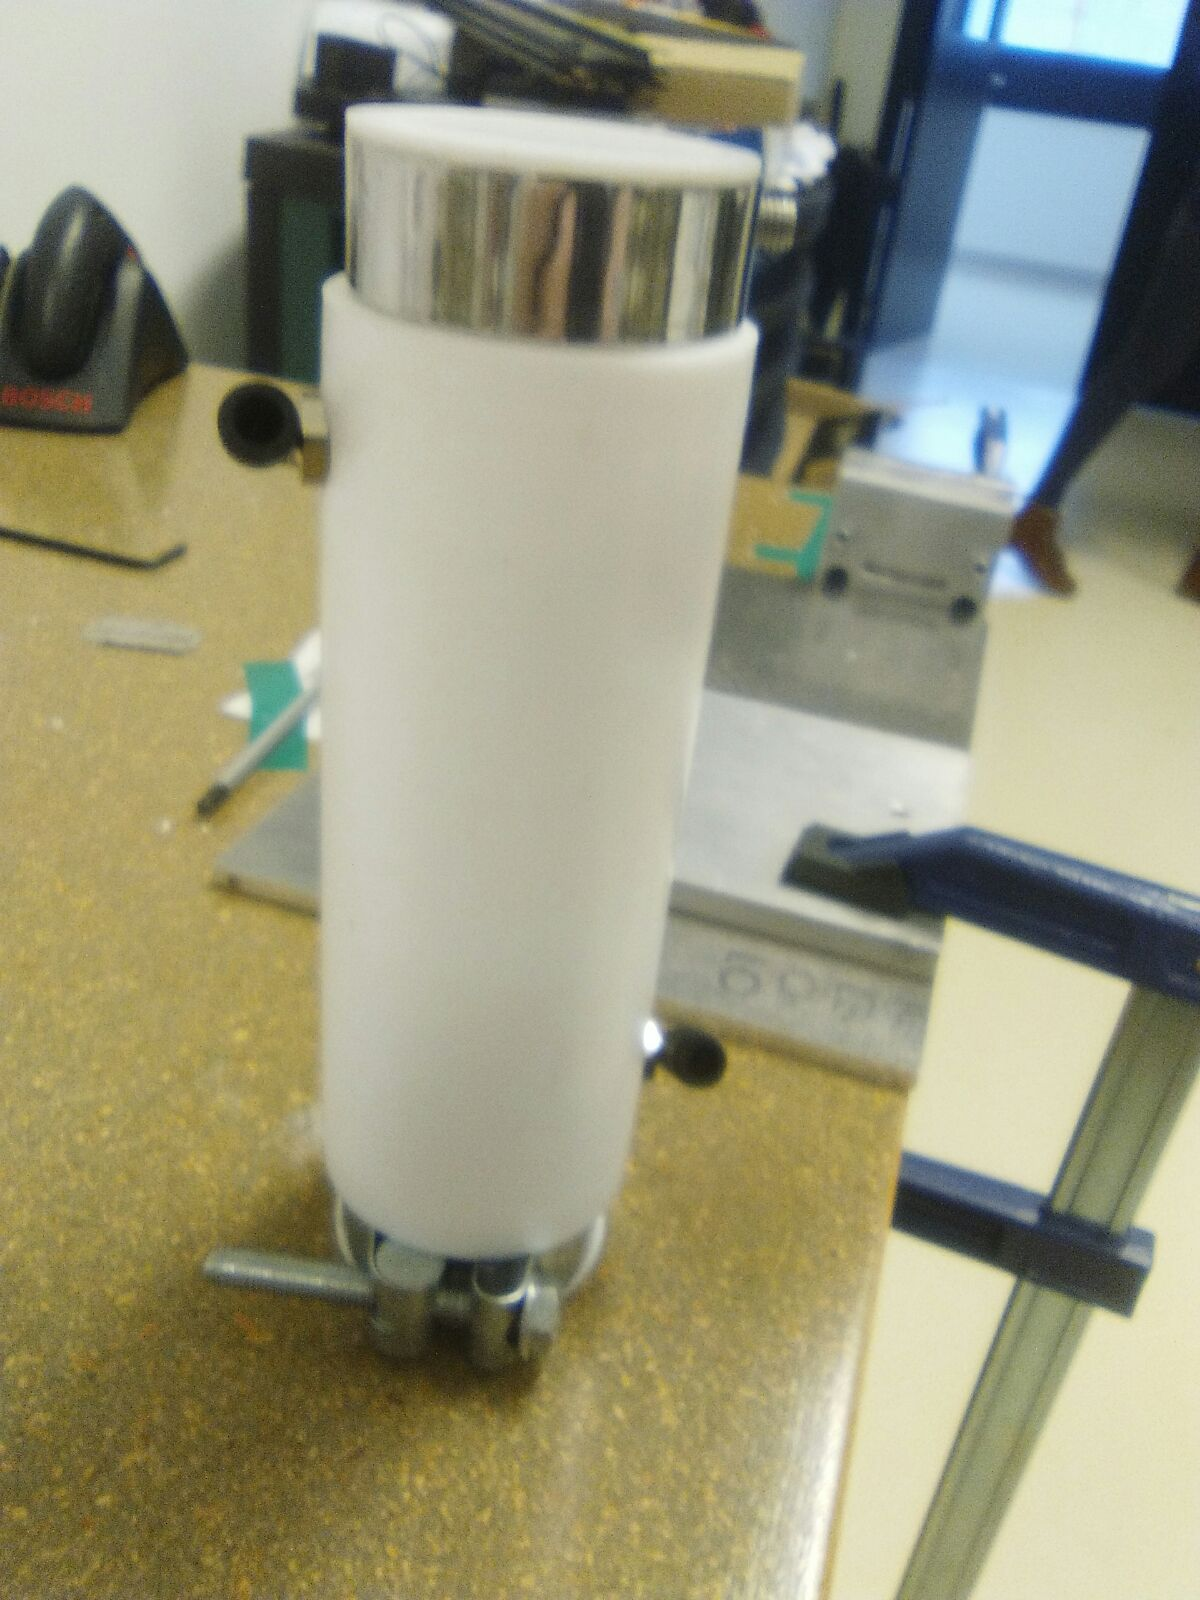
\includegraphics[scale=0.2]{Figures/AveiroPrototype.jpeg}
\end{figure}


\begin{Large}
\textbf{TRITIUM:}\\
\end{Large}
\begin{Large}
\textbf{Aveiro prototype}\\
\end{Large}
\vspace*{0.2in}
\today 
\paragraph {}
\begin{large}

\begin{multicols}{3}

\small João Veloso\\
(Universidad de Aveiro)\\
e-mail:joao.veloso@ua.pt\\
\vspace{1cm} 

Carlos Acevedo\\
(Universidad de Aveiro)\\
e-mail: cdacevedo@ua.pt\\
\vspace{1cm} 

Marcos Martinez Roig\\
(Universidad de Valencia)\\
e-mail: marcos.martinez@ific.uv.es

\end{multicols}

\end{large}
\vspace*{0.3in}
\rule{80mm}{0.1mm}\\
\vspace*{0.1in}
Tritium report\\
Department: nuclear and particle physics\\
\end{center}
\end{titlepage}

%\newpage
\tableofcontents
\newpage

%%%%%%%%%%%%%%%%%%%%%%%%%%%%%%% MAIN BODY %%%%%%%%%%%%%%%

%\newpage
\section{Introducción} \label{sec:Introduccion}
En este trabajo se ha realizado en el marco del proyecto Tritium. Su objetivo es realizar una caracterización de las fibras, modelo BCF-12, de Saint-Gobain. A pesar de que para el proyecto Tritium únicamente es interesante las fibras sin clad, con el objetivo de obtener un estudio completo, este estudio se ha extendido también para las fibras single clad y multi clad por completitud.

La diferencia entre estos tres tipos de fibra esta en que la no clad esta formada únicamente por un nucleo de poliestileno con un indice de refracicón de $1.60$ mientras que, en la single clad, el nucleo se encuentra recubierto por un material acrilico con un grosor de $30~\mu\meter$ y con un índice de refracción de $1.49$, un índice menor para asegurar la reflexión de los fotones por encima de un cierto ángulo con la superficie (ley de Snell) y, de esta forma, aumentar la recolección de luz. Finalmente las fibras multiclad se encuentras recubiertas por un segundo clad formado por un material Fluor-acrilico de un grosor de $10~\mu\meter$ y con un índice de reflacción de $1.42$, nuevamente inferior al índice del primer clad por la misma razon, aumentar la recolección de luz todavía mas.

La manera de realizar este exprimento será medir la eficiencia de colección de las fibras (en número de fotones por nanosegundo) para cada uno de los tipos de fibra anteriormente mencionados. Ello se realizará a traves de la siguiente expresión:

\begin{equation}
N.\gamma/~\nano\second=(I_{PMT}-I_{DC})10^{-9}/\epsilon/e
\label{intensidad}
\end{equation}


donde:
\begin{itemize}
\item{} $N.\gamma/~\nano\second$ es la eficiencia de colección, 
\item{} $I_{PMT}$ y $I_{DC}$ es la señal de intensidad medida en amperios obtenida de cada fibra cuando estamos alimentando la LED del sistema y cuando no, respectivamente. Esta señal se obtiene con ayuda de un tubo fotomultiplicador Hamamatsu R8520-ZB2771, el cual se encuentra en el laboratorio de reacciones nucelares y esta caracterizado y bien conocido. Esta señal se lee directamente con un picoamperímetro que promedia sobre N muestras (N=100 para nuestro estudio).
\item{} $\epsilon$ es la eficiencia del fotomultiplicador empleado, para nuestro caso $29.76\%$
\item{} $e$ es la carga del electrón.
\item{} el factor $10^{-9}$ aparece debido al cambio de unidades.
\end{itemize}

También se pretende determinar la desviación estandar asociada al proceso de preparación de cada fibra, $\sigma_{int}$, el cual estará presente en el experimento Tritium. Esta es una incertidumbre inerente en nuestro experimento debido al hecho de que cada fibra del detector Tritium necesita de un proceso de preparación que incluye tanto cortes con una guillotina especialmente fabricada en los talleres del IFIC, pulido con 5 hojas de diferente grosor, limpieza y tratamiento de las superficies de la fibra, etc. 

Sin embargo, hay que tener en cuenta que el sistema que se ha diseñado para medir estas magnitudes posee en todo momento una incertidumbre adicional debida a la posición de la fibra en el mismo, $\sigma_{pos}$. Dado que se trata de incertidumbres no correlacionadas podemos expresar esto con la siguiente ecuación matemática:

\begin{equation}
\sigma_{total}=\sqrt{\sigma_{pos}^2+\sigma_{int}^2}
\label{dispersiontotal}
\end{equation}

donde $\sigma_{total}$ es la incertidumbre que medimos en un experimento.

Por tanto, dado que únicamente nos interesa determinar la incertidumbre asociada al proceso de fabricación ya que es la única que intervendrá en el proyecto Tritium, para poder medir esta necesitamos diseñar dos experimentos:
\begin{itemize}
\item{} Un primer experimento en el que no contribuya la incertidumbre debida al proceso de fabricación $\sigma_{int}=0$ y que, por tanto, nos permita cuantificar la desviación estandar debida a la posición de la fibra:
$$\sigma_{total}=\sigma_{pos}$$
\item{} Un segundo experimento en el que si contribuya la incertidumbre debida al proceso de fabricación (y la debida a la posición de la fibra, la cual es inevitable). Este estudio nos permitirá cuantificar $\sigma_{total}$ para cada tipo de fibra, cuya expresión corresponde a la expresión \ref{dispersiontotal} y, conocida $\sigma_{pos}$ del estudio anterior, podremos extraer el valor de $\sigma_{int}$ como:

\begin{equation}
\sigma_{int}=\sqrt{\sigma_{total}^2-\sigma_{pos}^2}
\label{incertidumbreint}
\end{equation}
La cual, como hemos dicho, es la única incertidumbre interesante desde el punto de vista del proyecto Tritium.
\end{itemize}


%\newpage
\section{Dispostivo experimental} \label{sec:SetUp}
El dispostivo experimental diseñado para la realización del estudio de caracterización de estas fibras se muestra de forma esquemática en la figura \ref{esquemasetup}.

\begin{figure}[H]
\centering
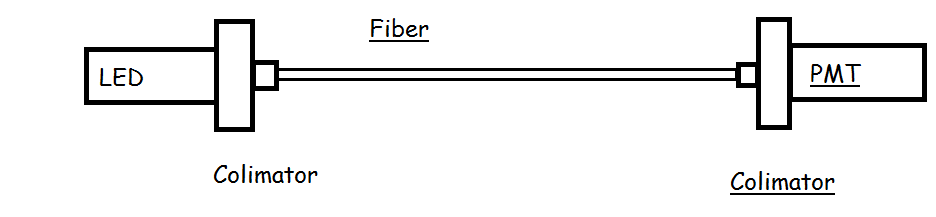
\includegraphics[scale=0.45]{Figuras/Set_up.png}
\caption{Esquema del dispositivo experimental utilizado en el estudio\label{esquemasetup}}
\end{figure}

El dispositivo esperimental esta formado por 5 piezas distintas:
\begin{itemize}
\item {} En primer lugar podemos observar la existencia de un diodo LED, el cual actuará como fuente de fotones. Con ayuda de un espectrómetro existente en los laboratorios del ICMOL se ha realizado un espectro de los fotones emitidos por el diodo LED el cual puede observarse en la figura \ref{espectroled}

\begin{figure}[H]
\centering
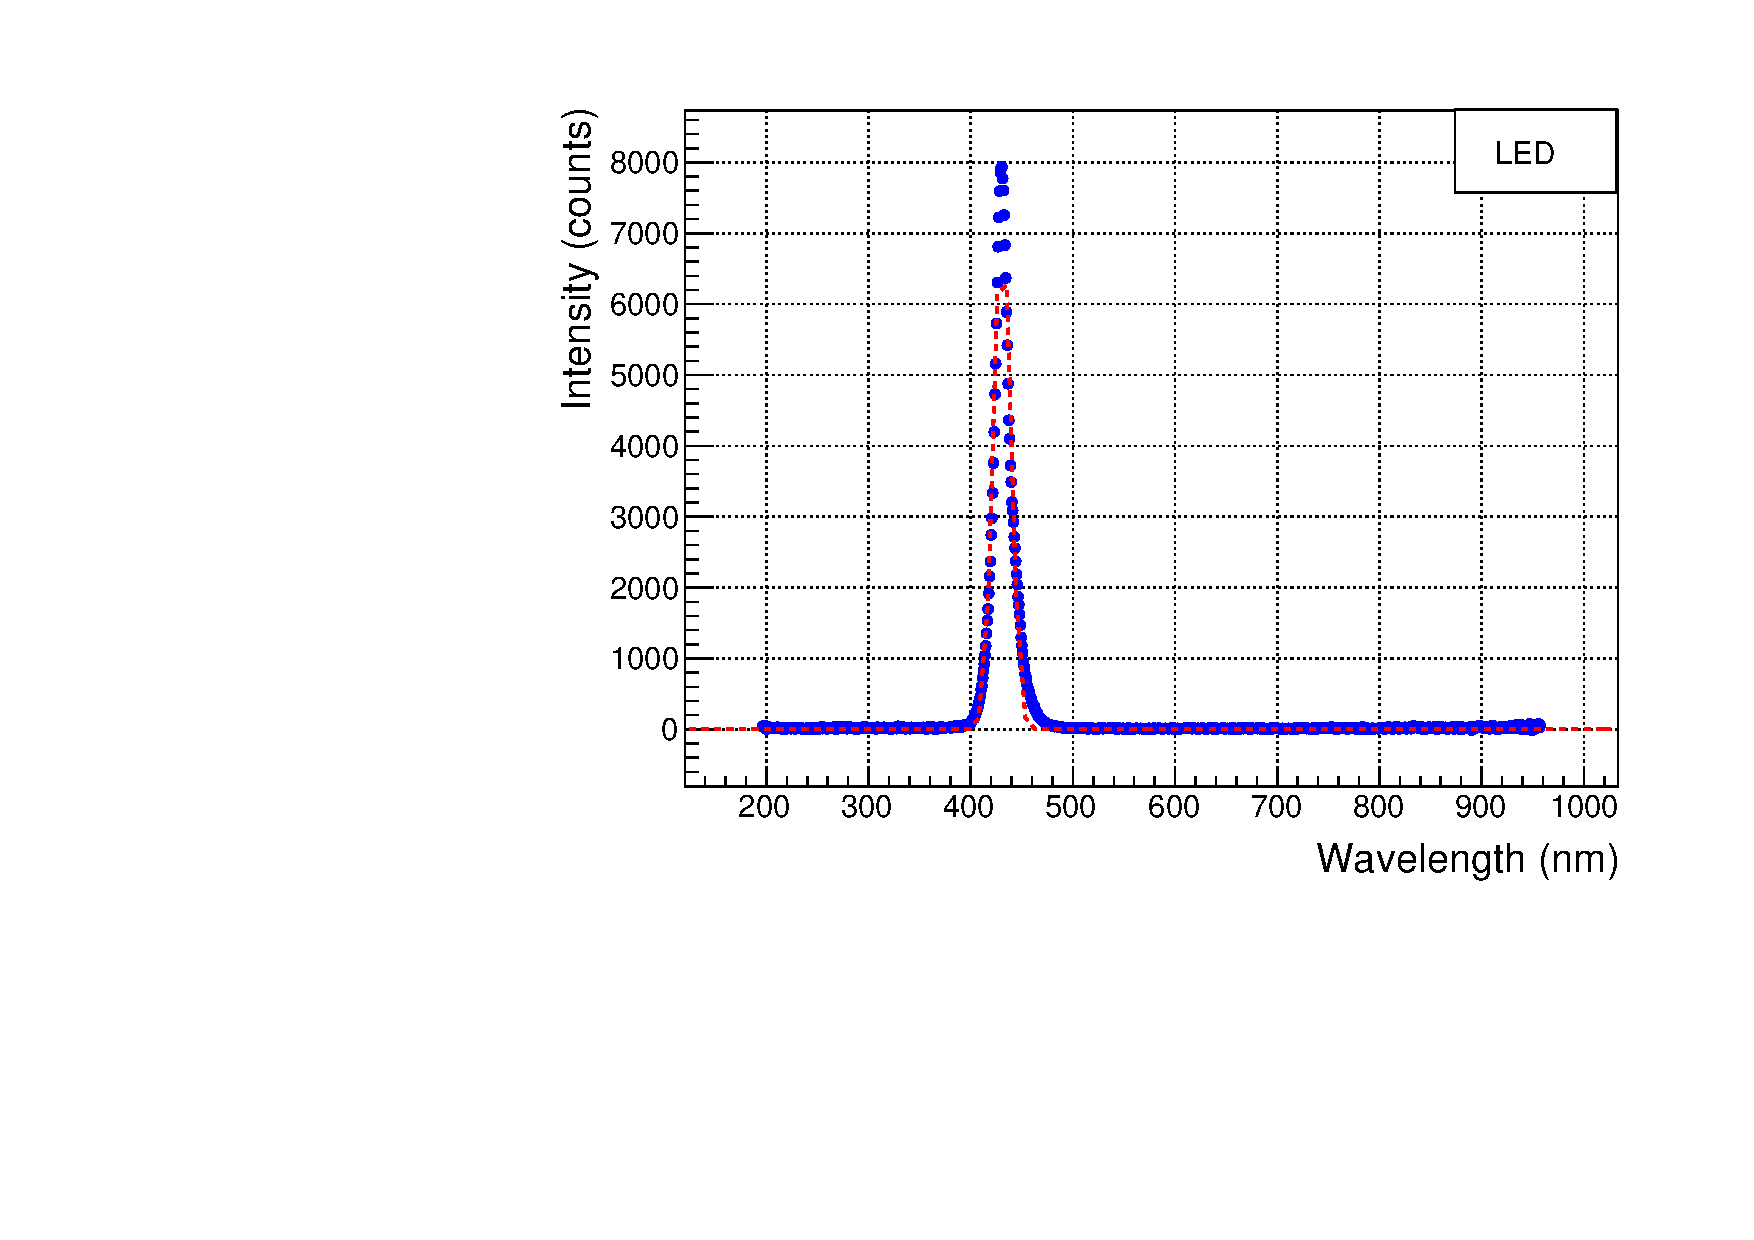
\includegraphics[scale=0.7]{Figuras/Plot_LED.pdf}
\caption{Espectro del diodo LED empleado en el dispositivo experimental\label{espectroled}}
\end{figure}

En este podemos comprobar que la emisión del diodo led posee un pico bastante estrecho el cual, con ayuda de un ajuste a una gaussiana, observamos que se encuentra en $\lambda=430,8 \pm 0.1$ con una anchura de $\sigma_{\lambda}=8.3\pm0.1$. La razón de ello es que queremos caracterizar las fibras en este intervalo del espectro debido a que este es el intervalo de interes desde el punto de vista del proyecto Tritium ya que nos encontramos muy cerca del pico de emisión que presentan la fibras empleadas en el estudio (BCF-12), el cual se encuentra entorno a $\lambda=435~\nano\meter$.

\item{} Un tubo fotomultiplicador (PMT) con el que leeremos el número de fotones que recibamos del sistema. El PMT utilizado es Hamamatsu R8520-ZB2771, cuya eficiencia a la longitud de onda de trabajo es de $\epsilon=29.76\%$. Este se encuentra alimentado a $250~\volt$ y posee un cortocircuito en el sistema de dinodos que le permite acturar con ganancia 1.

\item{} La fibra sometida a estudio se situará entre ambos dispositivos anteriormente mencionados, el diodo LED y el PMT. El objetivo de este es que la señal que midamos provenga de los fotones emitidos por el diodo LED tras haber cruzado la fibra centelleadora. Dado que con el estudio anterior sober el diodo LED tenemos bien caracterizada su señal, con este sistema podremos quantificar la eficiencia de colección que presenta cada tipo de fibra ademas de sus posibles incertidumbres procedentes de diversas fuentes.

Hay que tener en cuenta que la longitud activa de la fibra en la que se estudiará la caracterización de estas es lijeramente menor que la longitud total. El motivo de ello es que una pequeña parte de estas (aproximadamente $4~\mm$ a cada lado) son empleados para cruzar el conector y realizar un contacto opticamente aceptable con el PMT con ayuda de grasa óptica. Estas pequeñas longitudes se encuentran recubiertas por finas capas de teflón (politetrafluoroetileno) el cual posee un coeficiente de reflexión de prácticamente el $100\%$ con fotones en el rango del visible, com es nuestro caso. Esto se realiza para evitar añadir la incertidumbre del tramo del interior del conector ya que estos son metálicos y solo nos interesa realizar la caracterización en un medio aéreo. En trabajo, siempre que hablemos de longitud, nos estaremos refiriendo a la longitud activa de la fibra. En caso contrario se especificará.

\item{}Seguidamente queremos asegurar que los fotones medidos por el tubo fotomultiplicador procedan únicamente del diodo LED tras haber cruzado la fibra. Para ello introducimos un primer colimador justo antes del PMT, de esta manera seguramos que los fotones que medimos proceden del interior de la fibra y un segundo colimador justo despues de la LED. Con esta configuración podemos asegurar que la procedencia de estos fotones es la adecuada. Ambos colimadores han sido específicamente construidos en los talleres del IFIC para este estudio por lo que posee una colimación perfecta.

\item{} Finalmente se emplearan unos conectores comerciales obtenidos de la empresa Saint-Gobain para sujetar de forma segura estas fibras, tanto en el dispositivo experimental como en las diversas labores que así lo requieran como por ejemplo el pulido. Estos conectores pueden verse en la figura \ref{conector}.

\begin{figure}[H]
\centering
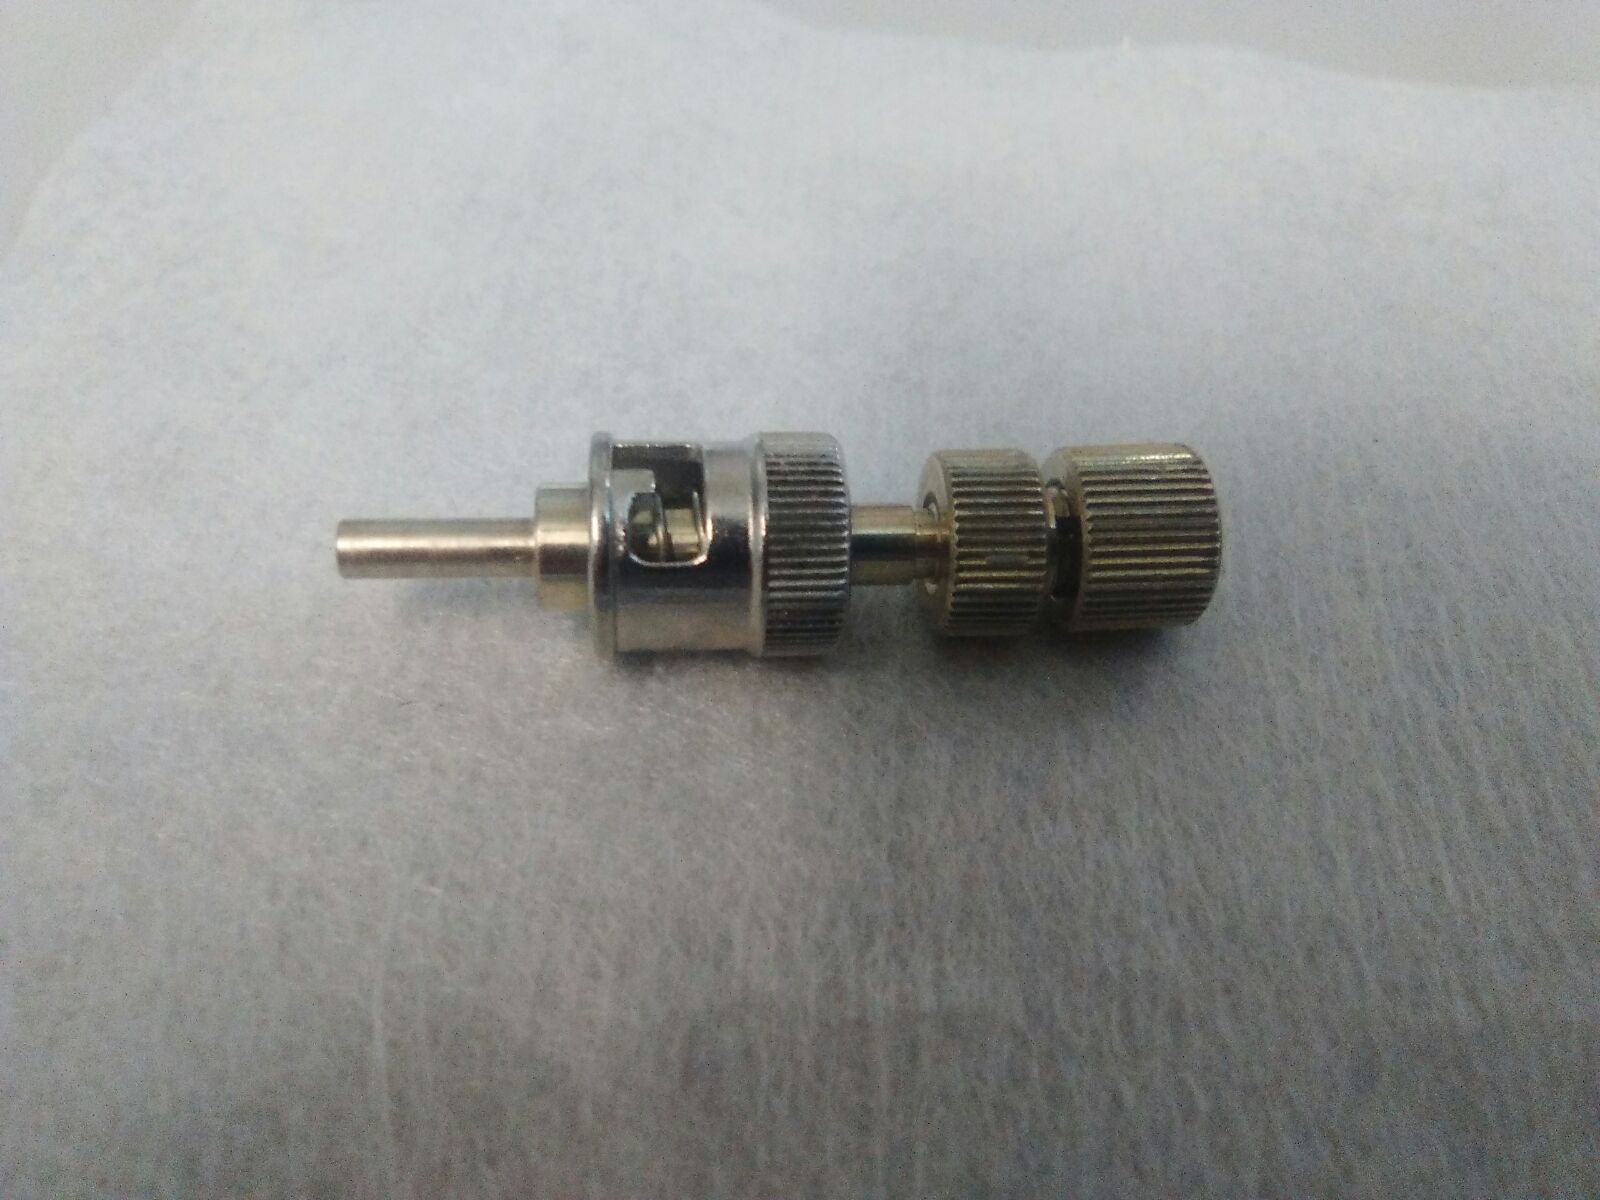
\includegraphics[scale=0.1]{Figuras/conector.jpeg}
\caption{Conector comercial empleado para la sujeción de la fibra\label{conector}}
\end{figure}

Hay que tener en cuenta que, dado que estos conectores son metálicos, se utilizaron finas capas de teflón entre la fibra y el conector para evitar daños en la fibra.




\end{itemize}


%\newpage
\section{Preparación del dispositivo} \label{sec:Preparacion}
En primer lugar, antes de empezar con el estudio de la caracterización de las fibras, necesitamos realizar una serie de labores de preparación del dispositivo experimental para asegurar el correcto funcionamiento y entendimiento del mismo. Para ello realizaremos tres comprobaciones:
\begin{itemize}
\item{} En primer lugar, realizaremos una comprobación para asegurar que el diámetro de las fibras se corresponde con el proporcionado por la empresa Saint-Gobain.

\item{} En segundo lugar realizaremos una estudio para verificar la hermiticidad a la luz de la caja oscura en el interior de la cual se desarrollará el estudio.

\item{} En último lugar realizaremos un estudio del PMT utilizado en el experimento para asegurar la linealidad de su respuesta del mismo en el intervalo de interes en el experimento y, en concreto, en el detector Tritium ya que, aunque su iniciativa primera será utilizar SiPM también se estudiará la posibilidad de emplear PMTs.
\end{itemize}

	%\newpage
	\subsection{Comprobación del diámetro de las fibras utilizadas} \label{sec:Diametro}
	Procedemos a comprobar el diámetro de las mismas cuyo valor proporcionado por Saint-Gobain es de $1~\mm$. Para ello medimos el diámetro de 3 fibras diferentes de cada tipo con ayuda de un microscopio electrónico del ICMOL, cuya incertidumbre se encuentra entorno al nanómetro. Los resultados promediado se muestra en la tabla \ref{diametros} .

\begin{table}[H]
\begin{center}
\begin{tabular}{l | c | c | c | c }
Tipo de fibra & Electronical microscope $(\sigma_{el}\approx 10^{-6} mm)$\\
\hline \hline
No Clad (mm)& $1.00 \pm 0$\\ 
Single clad (mm) & $1.00 \pm 0$\\
Multi clad (mm)  & $1.00 \pm 0$\\
\end{tabular}
\caption{Diámetro promediado sobre tres muestras\label{diametros}}
\end{center}
\end{table}

Podemos apreciar que el diámetro de todas las fibras que se midieron fue exactamente un milímetro con una resolución de $10^{-6}~\mm$ ofrecida por el microscopio electrónico ya que la desviación estandar del promedio es exactamente cero. 

Con este estudio se ha comprobado que la adición de clad implica la retirada de núcleo centelleador, es decir, Saint-Gobain ofrece una mejora en la colección de luz a costa de un menor núcleo centelleador. 

Hay que tener en cuenta que esta retirada de núcleo centelleador no afecta al proyecto Tritium ya que los electrones procedentes de la desintegración del tritio, y que aportarán señal de forma apreciable, únicamente recorrerán un máximo de 5 o 6$~\mu\meter$ y, incluso con los multiclads, la fibra posee un núcleo de mas de $900~\mu\meter$ de diámetro. El problema aparece únicamente con los clads comerciales ya que estos poseen un espesor mínimo de $40~\mu\meter$, por lo que, si tenemos en cuenta el recorrido libre medio de estos eventos, podemos ver que ninguno conseguirá llegar al núcleo de la fibra y aportar señal al detector. Se esta estudiando la posibilidad de crear núcleos que permitan la recolección total de los fotones pero lo suficientemente finos para que no afecten de forma importante a la tasa de eventos de tritio que consigan llegar al nucleo.
	
	%\newpage
	\section{Comprobación de la hermiticidad a la luz de la caja oscura empleada en el estudio} 		\label{sec:manta}
	Ahora procedemos a comprobar la hermiticidad de la caja oscura en el interior de la cual se desarrollará el experimento. Para ello preparamos 3 muestras diferentes de fibras no clad de $200~\mm$ de longitud y realizamos una medición de cada una de estas para cuatro intensidades diferenets de alimentación de la LED. Seguidamenet repetimos el mismo experimento incorporando sobre el prototipo una manta oscura especial para asugurar la total hermiticidad del sistema a los fotones.

En la figura \ref{plotmanta} podemos observar las señales promediadas de ambos experimentos con su desviación estandar, la cual se muestra inapreciable a esta escala.

\begin{figure}[H]
\centering
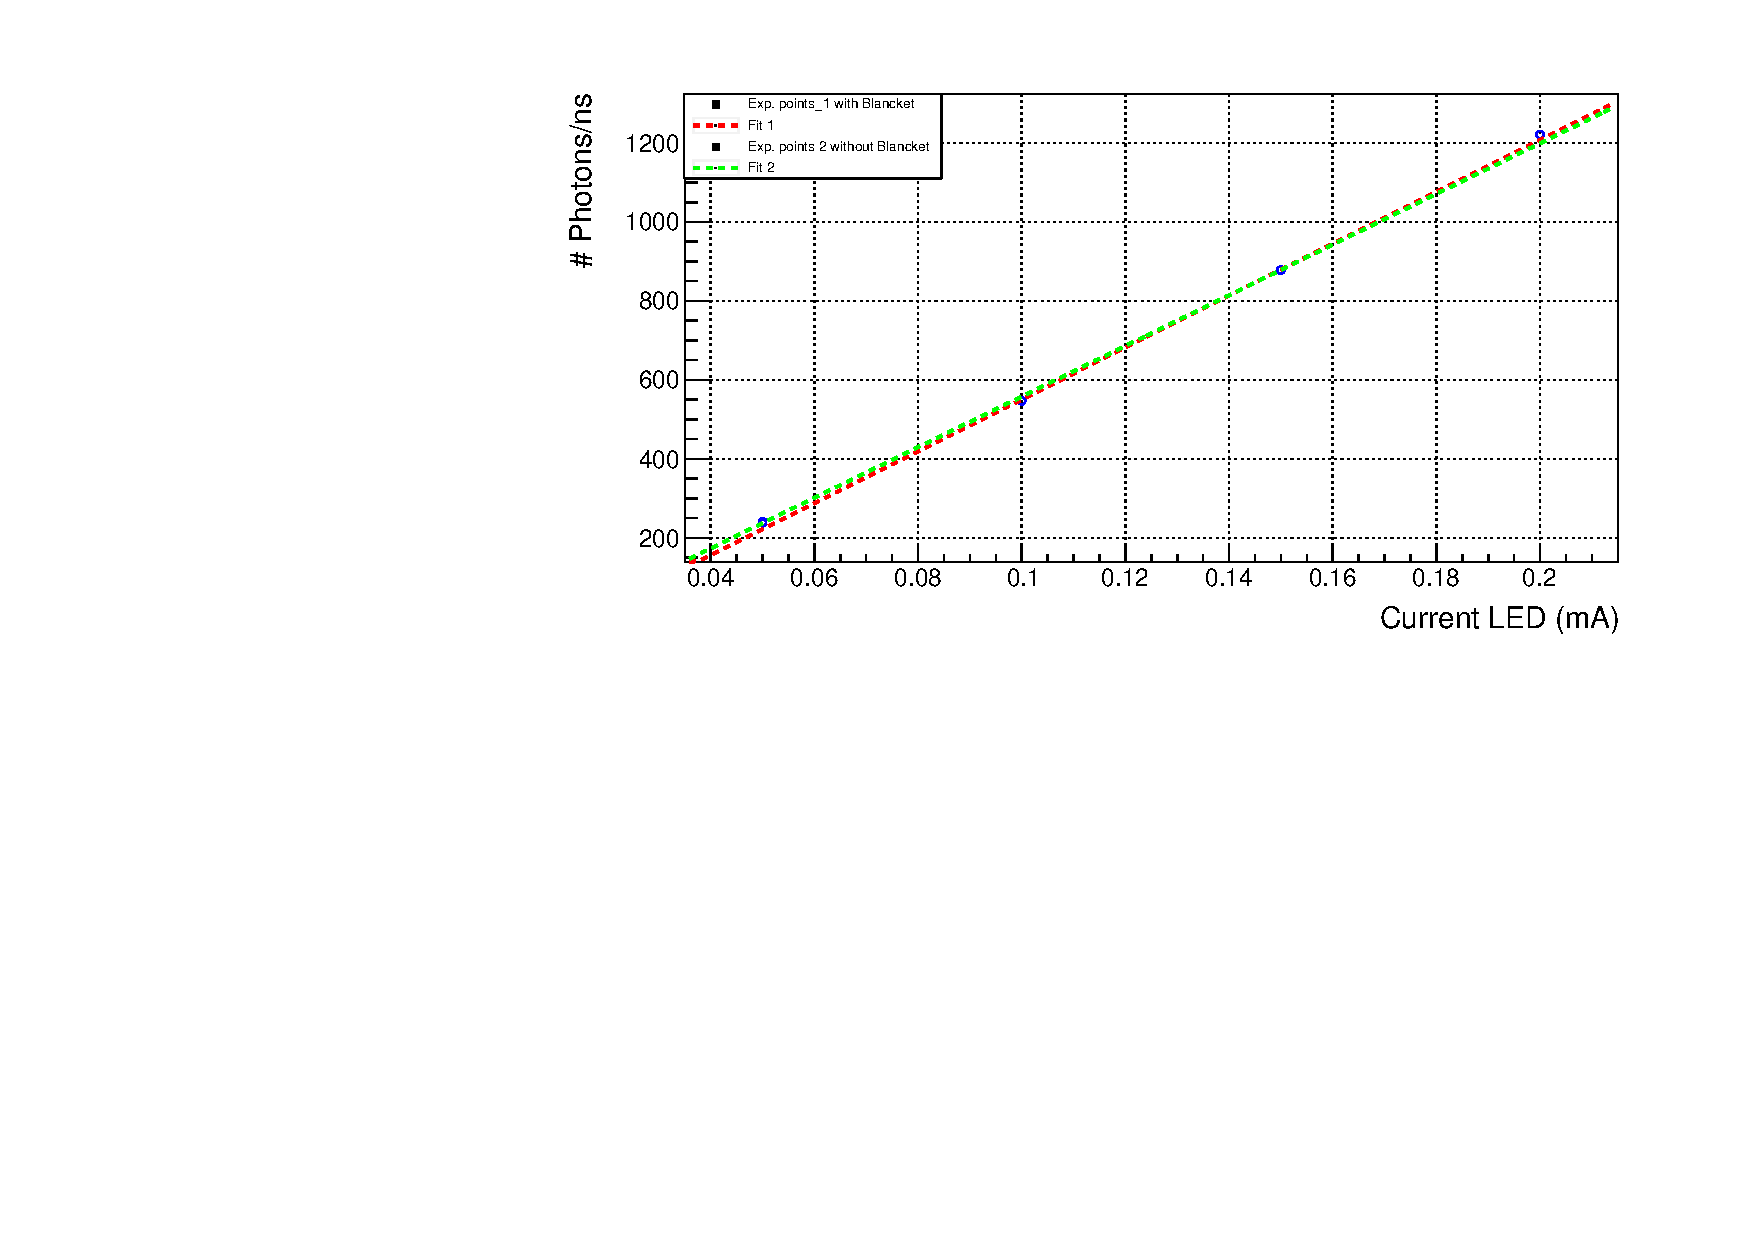
\includegraphics[scale=0.7]{Figuras/cases.pdf}
\caption{Señales medidas con y sin manta para fibras no clad de $200~\mm$\label{plotmanta}}
\end{figure}

Podemos observar que la señal es aproximadamente la misma. Finalmente representamos en la figura \ref{diferencia} la resta entre ambas señales.

\begin{figure}[H]
\centering
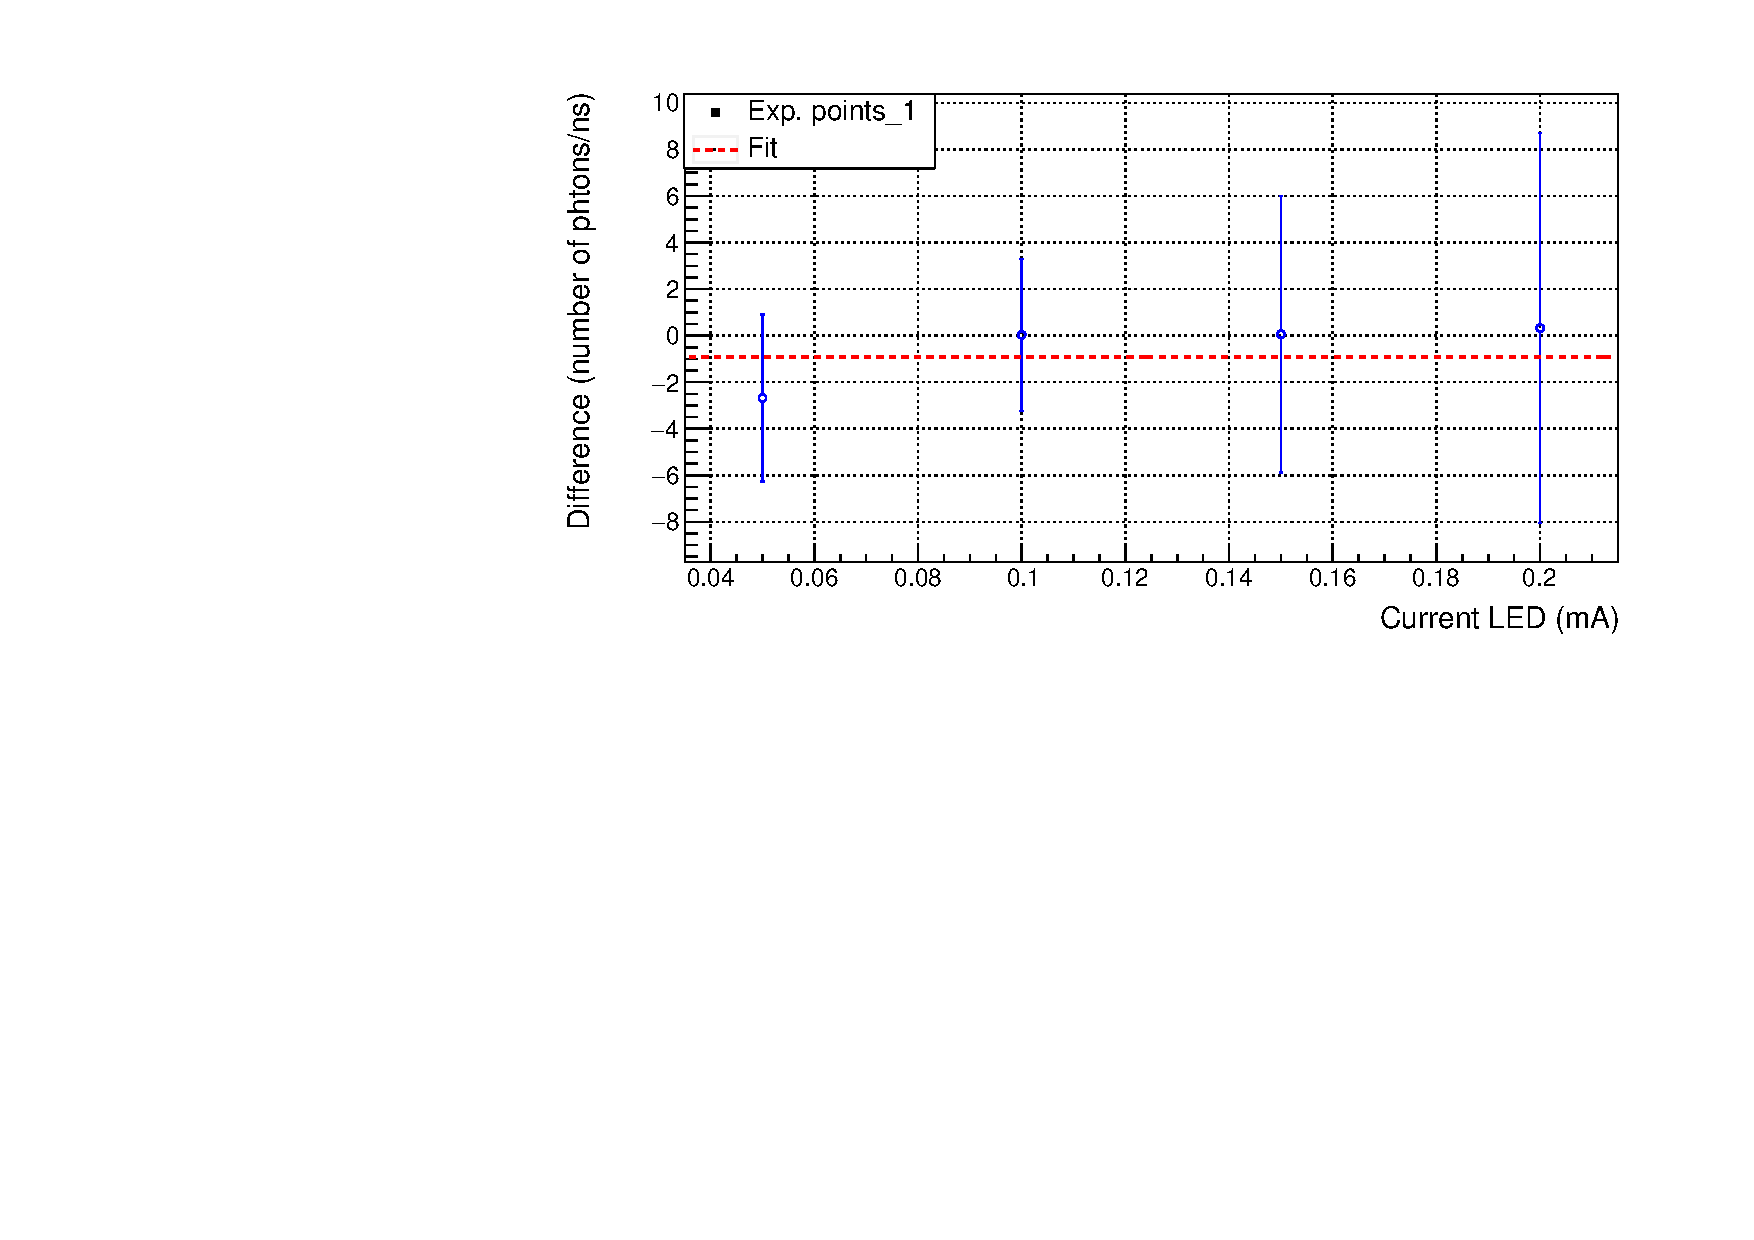
\includegraphics[scale=0.7]{Figuras/difference.pdf}
\caption{Diferencia entre las señales medidas con y sin manta para fibras no clad de $200~\mm$\label{diferencia}}
\end{figure}

Podemos observar que la diferencia es prácticamente nula. Con la propagación de incertidumbres vemos que las mínimas diferencias entres estas señales pueden explicarse perfectamente con la estadística. La razon de tener incertidumbres grandes es que este resultado se ha obtenido con la resta dos valores muy cercanos y muy grandes. Debido a ello tendremos errores superiores al valor numérico.





	%\newpage
	\subsection{Estudio de la linealidad del PMT} \label{sec:Linealidad}
	En último lugar realizaremos un estudio de la linealidad del PMT. 

En primer lugar buscamos testear esta linealidad al orden de número de fotones de un evento del agua tritiada ya que este será su objetivo final. Si tenemos en cuenta que, según el espectro de desintegración del tritio, sus eventos poseen una energía promedio de $5.7~\keV$ y que las fibras, según Saint-Gobain, poseen una eficiencia de fluorescencia de $8000~\gamma/\MeV$ para un mip (valor que se pretende comprobar en un futuro inmediato), podemos observar que un evento promedio del tritió corresponderá a $45$ fotones aproximadamente. Si tenemos en cuenta además la existencia de una lijera pérdida debido a la no existencia del clad en la fibra vemos que, este evento corresponderá a unas pocas decenas de fotones.

Para comprobar la linealidad del PMT a eventos de este orden utilizamos el dispositivo mostrado en la figura \ref{esquemasetup} donde situaremos el PMT a $200~\mm$ del diodo LED. Además, en este estudio no utilizaremos ninguna fibra y trabajaremos en el rango de linealidad del LED (alimentación hasta un máximo 5 amperios), de esta forma podemos asegurar que, en caso de producirse una no linealidad, esta será debida únicamente a la saturación del PMT. 

También utilizaremos colimadores para asegurar que la superficie activa con la que estamos leyendo es la del diametro de la fibra ya que, aunque un evento que no produzca saturación del PMT puede que, al reducir su superficie activa de detección, un evento de la misma energía si produzca saturación.

El resultado de este primer experimento se muestra en la figura \ref{linealidadordentritio}

\begin{figure}[H]
\centering
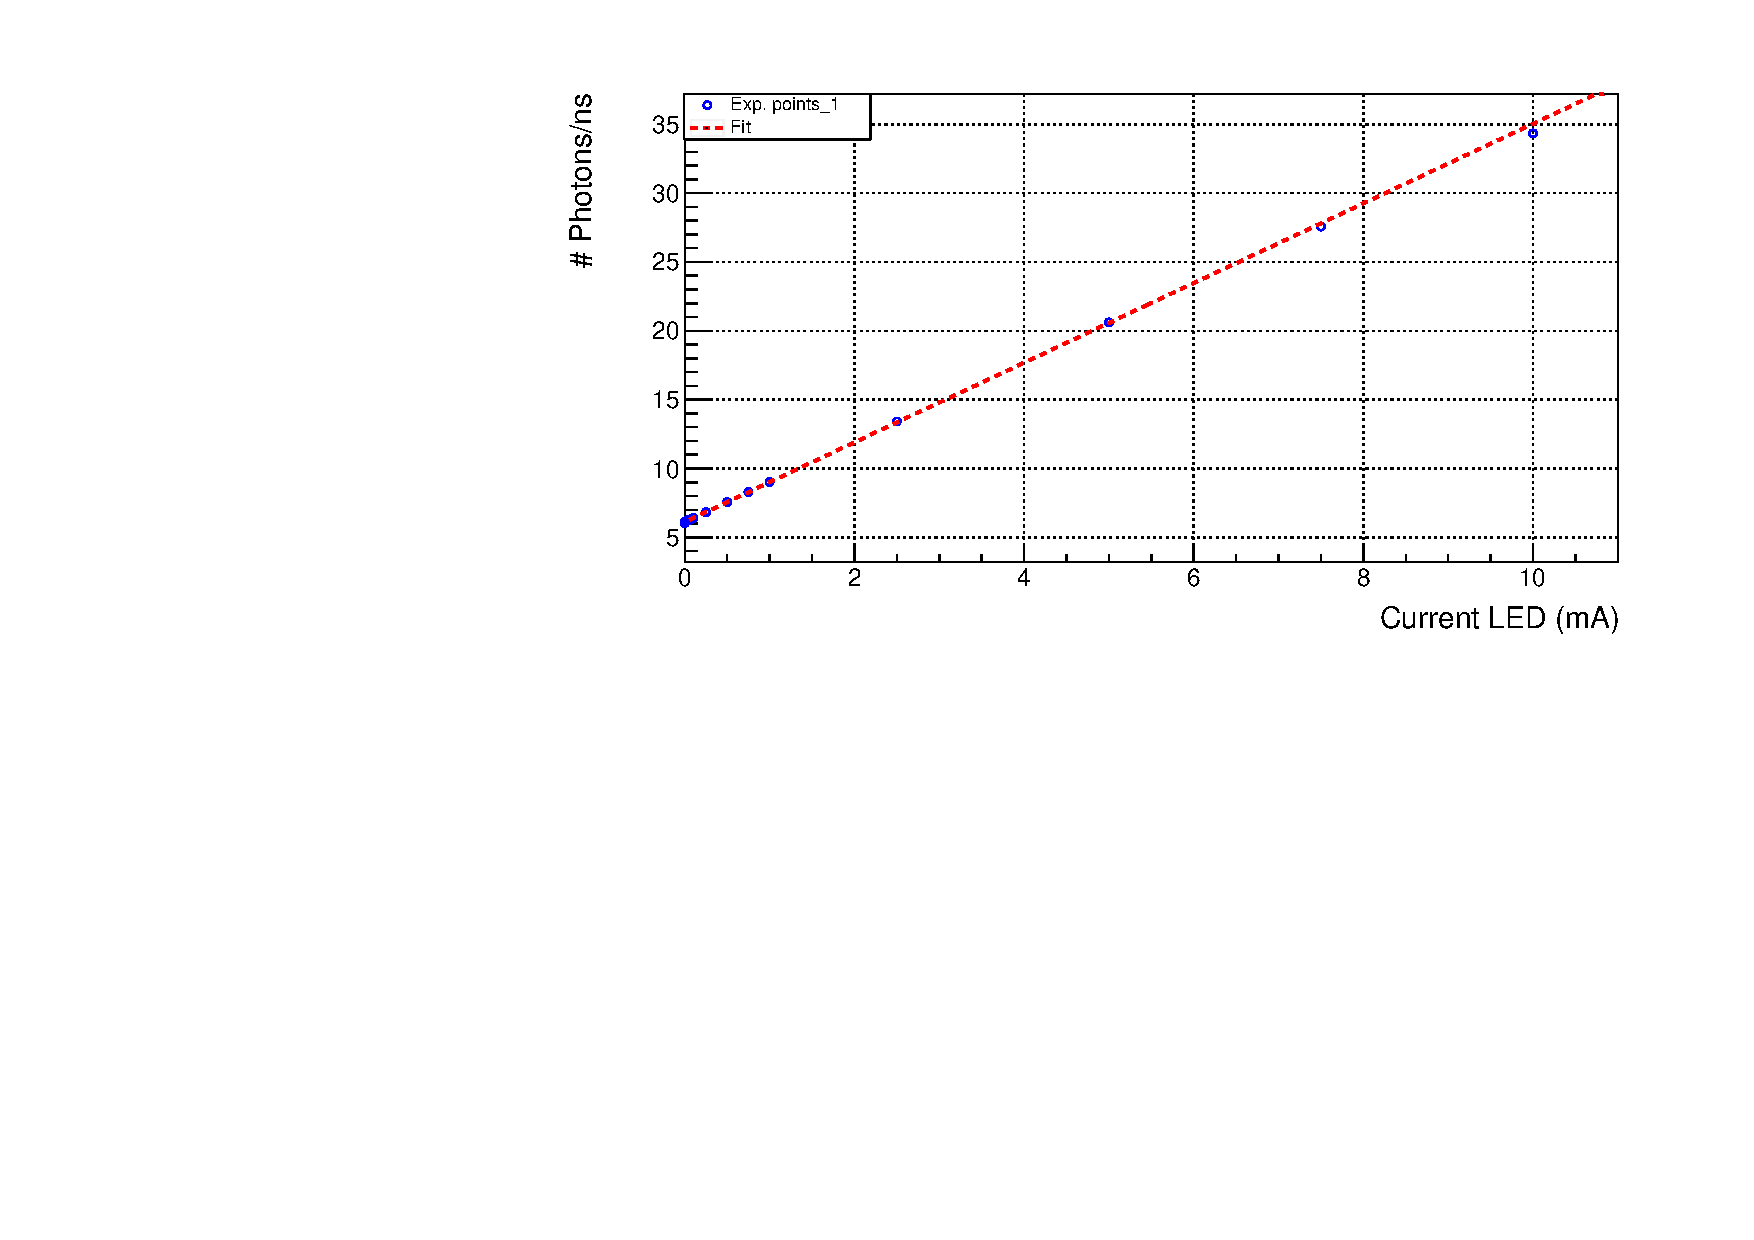
\includegraphics[scale=0.7]{Figuras/fit1background.pdf}
\caption{Respuesta del PMT utilizado en el experimento\label{linealidadordentritio}}
\end{figure}

Con esta gráfica podemos observar que, efectivamente, en el caso de que la actividad de la disolución de agua tritiada que pretendemos medir sea lo suficientemente baja para que el PMT no tenga pile-up este se comportará de forma perfectamente lineal, lo cual es fundamental si queremos realizar la monitorización de la actividad del tritio.

En la figura \ref{linealidadordentritio} puedo observarse que para intensidades de alimentación de la led muy bajas (inferior a $0.5~\milli\ampere$) se tomó un paso mucho menor. La figura \ref{zoomtransicion} muestra una ampliación de la región entre $0$ y $0.22~\milli\ampere$ y la figura \ref{zoomtransicion2} muestra una ampliación todavía mayor de la región entre $0$ y $0.005~\milli\ampere$.

\begin{figure}[H]
\centering
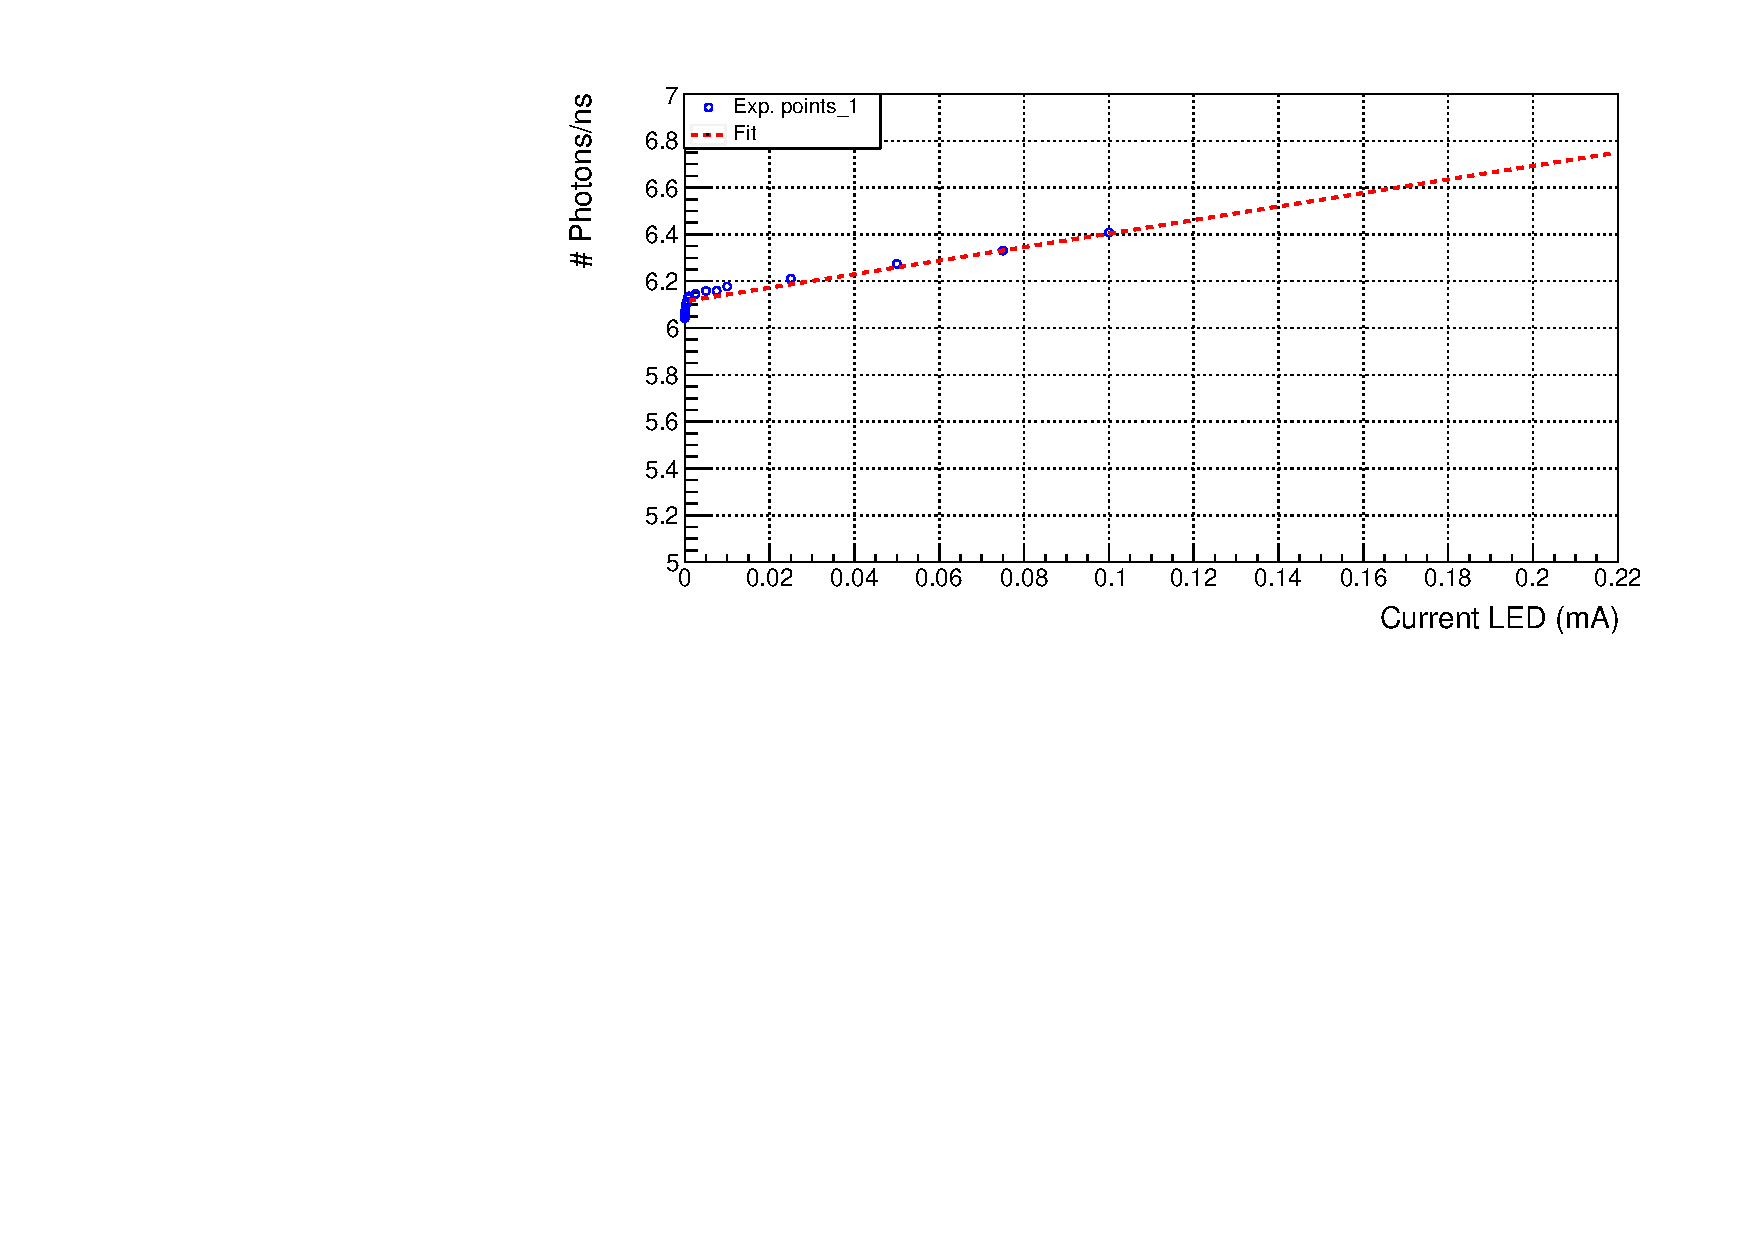
\includegraphics[scale=0.7]{Figuras/Transicionbackground.pdf}
\caption{Ampliación de la zona de transición\label{zoomtransicion}}
\end{figure}

\begin{figure}[H]
\centering
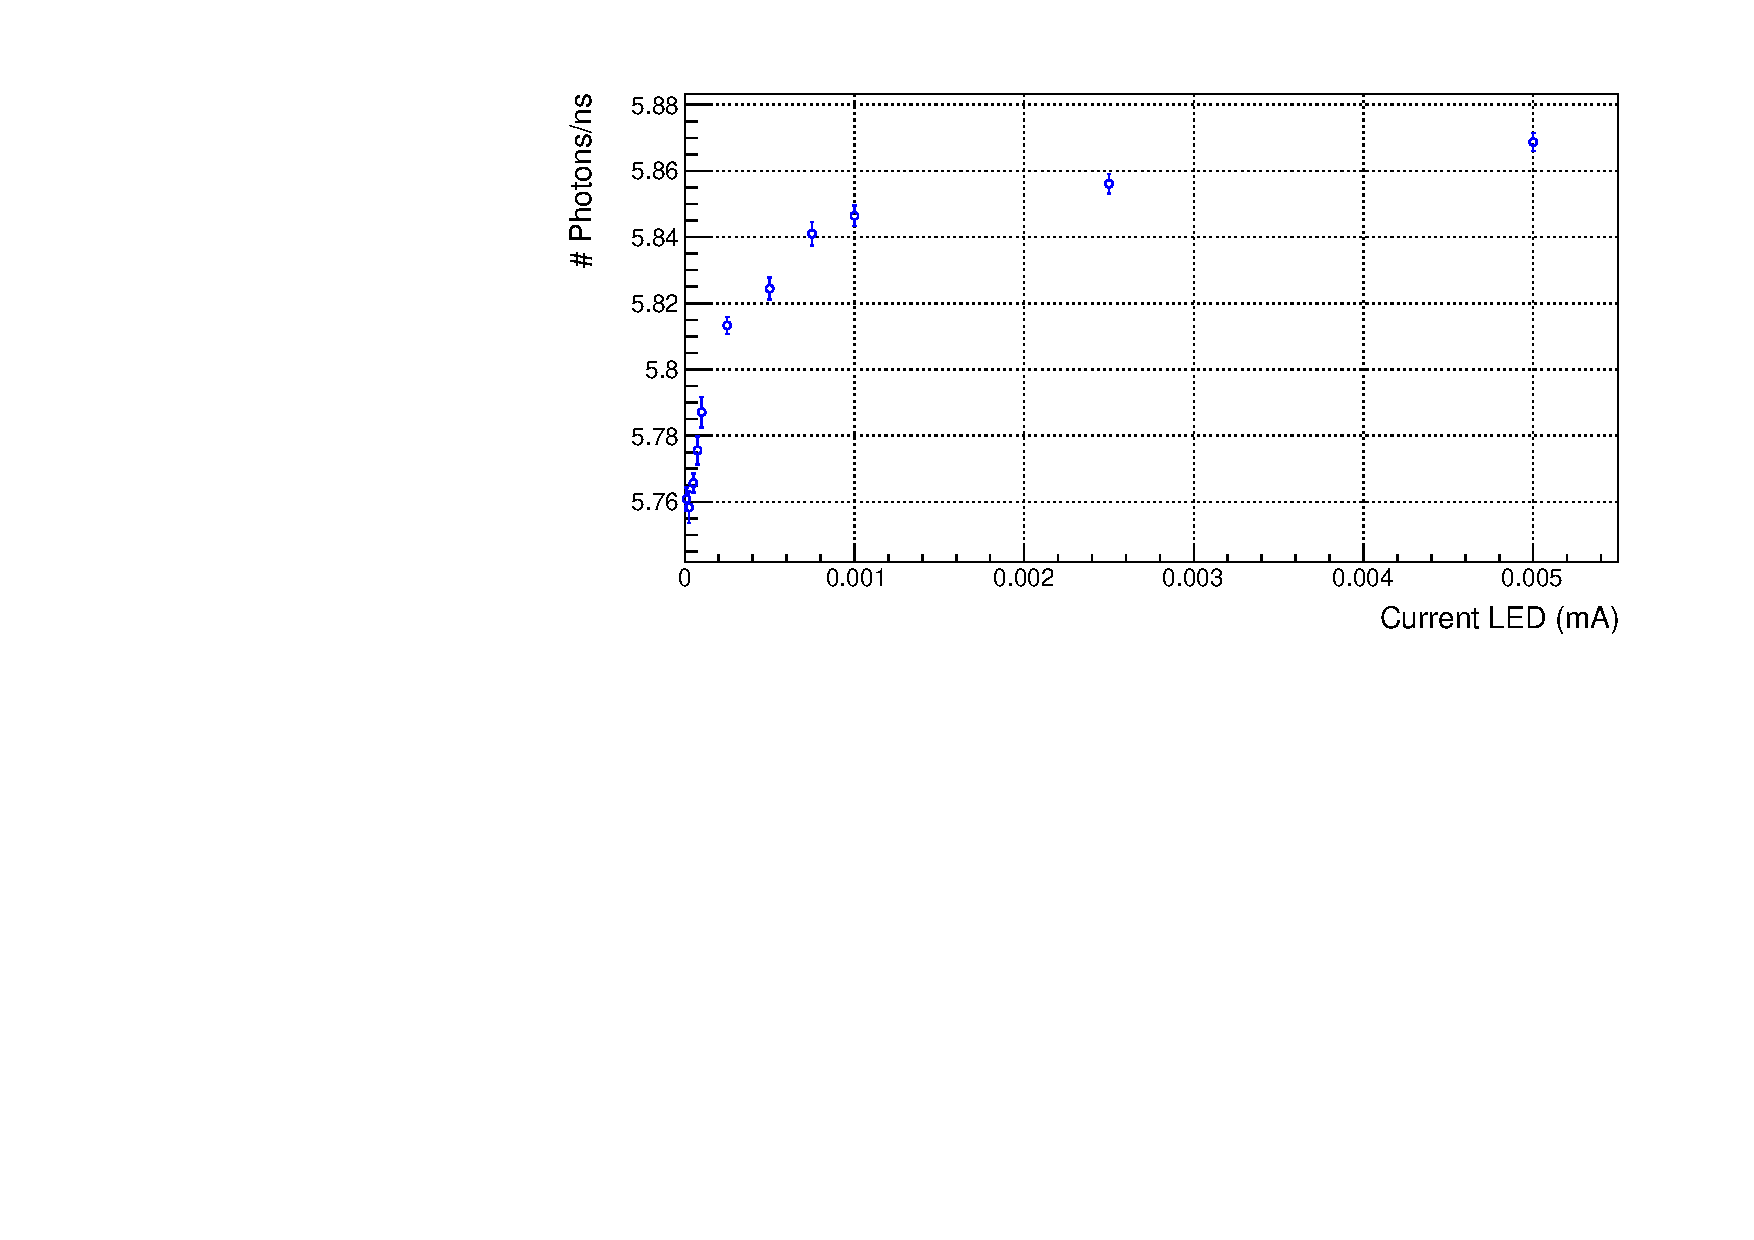
\includegraphics[scale=0.7]{Figuras/Transicionbackground2.pdf}
\caption{Ampliación de la zona de transición\label{zoomtransicion2}}
\end{figure}

Podemos observar que la existencia de una no linealidad en el comportamiento de nuestro sistema. Esto es debido al comportamiento de la LED cuya relación característia es:

\begin{equation}
I=I_s(e^{V_D/{nV_T}}-1)
\label{LED}
\end{equation}

Donde lo único que nos importa de esta expresión es que la dependencia entre la intensidad emitida por la led $I$ (número de fotones por unidad de tiempo) y el voltaje con el que esta se alimenta $V_D$ (el cual es proporcional a la intensidad con la que estamos alimentando) es una exponencial. Esta expresión, en primer orden de magnitud, puede aproximarse a una dependencia lineal. Este es el origen de la dependencia lineal entre la intensidad emitida por la LED y la intensidad con la que la alimentamos. Sin embargo, hay que tener en cuenta que el diodo LED consta de una unión PN de dos materiales semiconductores. Por ello, necesita alimentar con un voltaje mínimo (usualmente $V_{min}\approx 0.7~\volt$ para LEDs comerciales) a partir del cual los portadores de carga (electrones) tienen suficiente energía para pasar a la región de conducción. Es por ello que el diodo LED necesita un voltaje de alimentación mínimo (o, en nuestro caso, una intensidad de alimentación  mínima) para emitir fotones.

Realmente esta transición no es importante desde el punto de vista del proyecto tritium ya que este no utiliza el diodo LED. En el detector la fuente de fotones serán los diversos eventos de tritio capturados por las fibras. Además hemos visto que estos eventos tendrán del orden de unas pocas decenas de fotones donde, anteriormente, hemos comprobado que el sistema es lineal. 

Sin embargo es importante documentar esta púnto de mínima intensidad de alimentación de la LED ya que, para asegurar el correcto funcionamiento del sistema, debemos situarnos por encima de este punto, el cual, en la figura \ref{zoomtransicion2}, podemos ver que es $0.001~\milli\ampere$.

Finalmente, por completitud, extendemos el rango en dos ocasiones. En primer lugar lo extendemos hasta un máximo de $300~\gamma/\nano\second$, el cual puede verse en la figura \ref{300} y, en segundo lugar, lo extendemos hasta un máximo de $2500~\gamma/\nano\second$, el cual puede verse en la figura \ref{2500}

\begin{figure}[H]
\centering
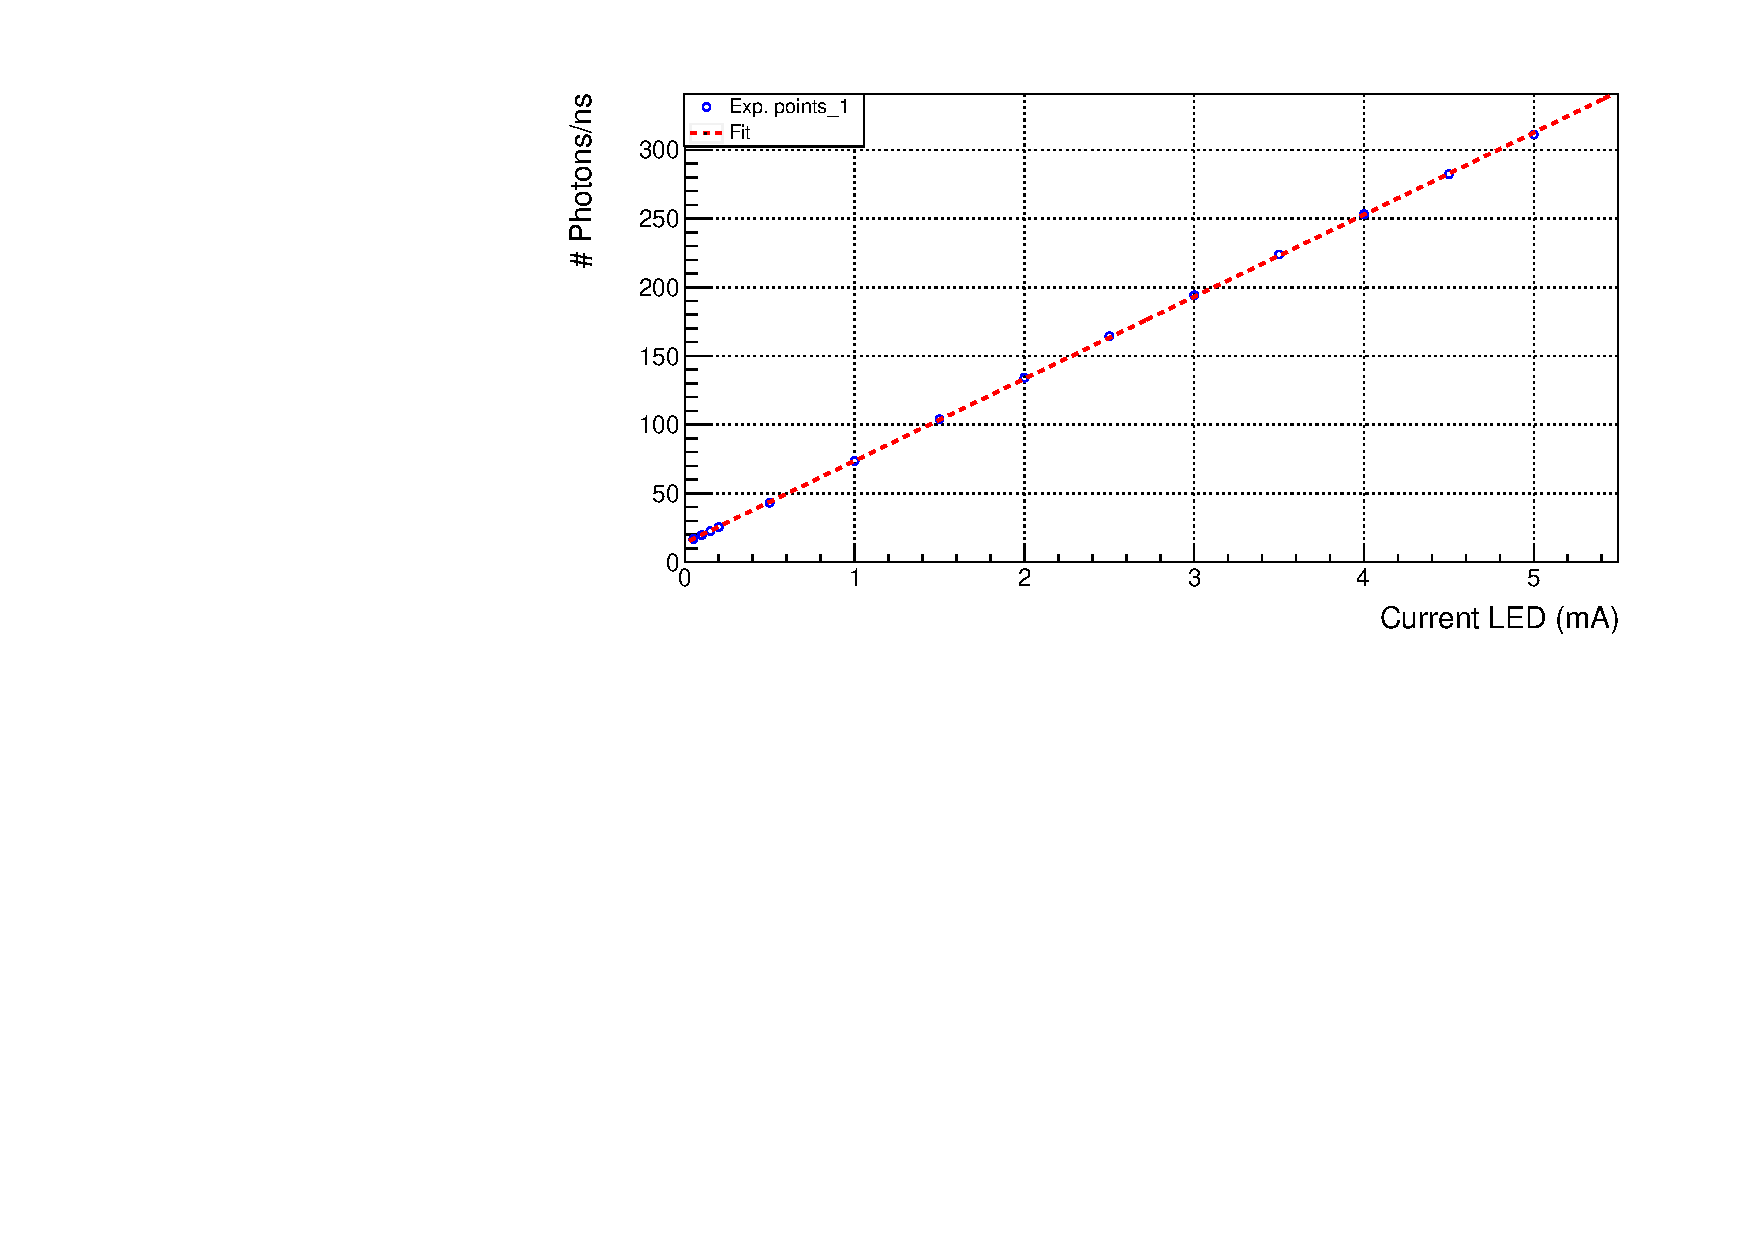
\includegraphics[scale=0.7]{Figuras/300.pdf}
\caption{Ampliación del intervalo de respuesta estudiado hasta 300 fotones por nanosegundo\label{300}}
\end{figure}

\begin{figure}[H]
\centering
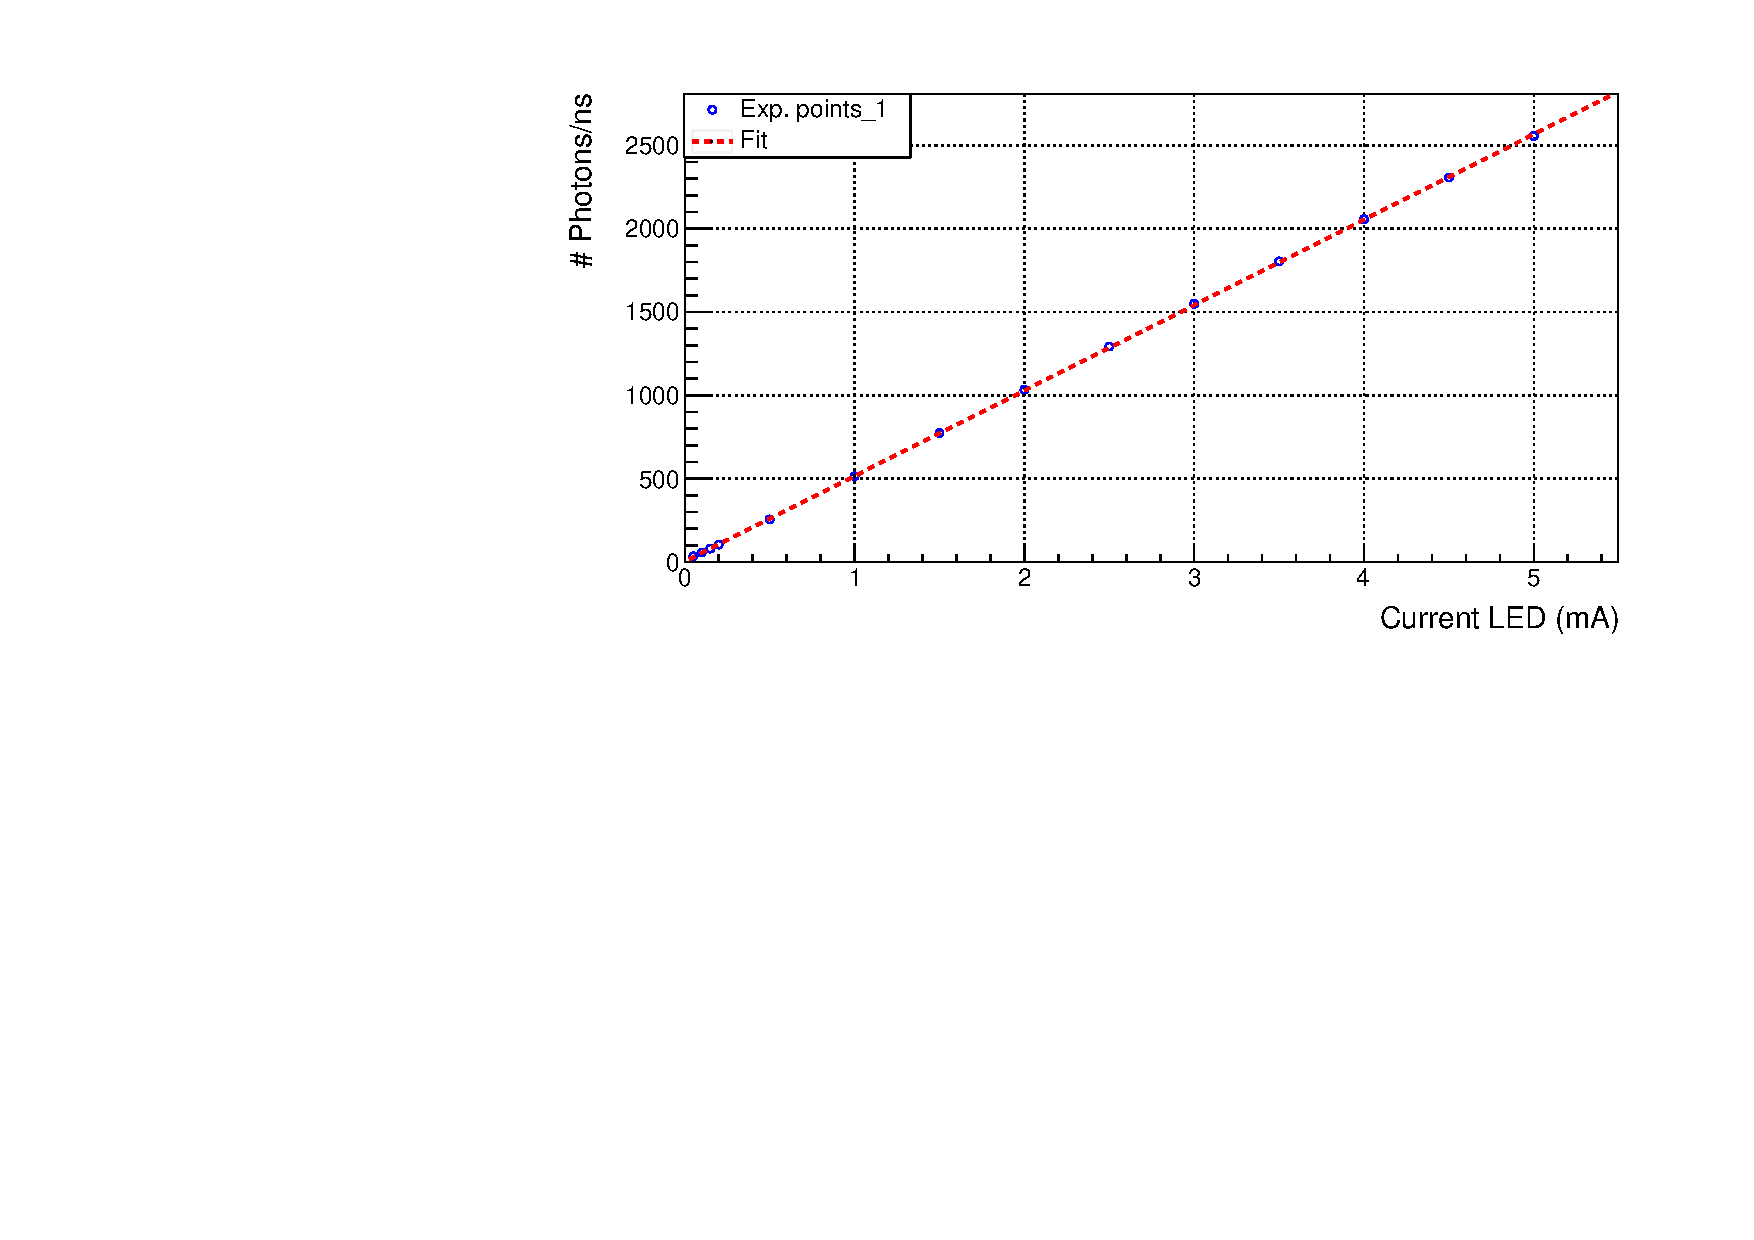
\includegraphics[scale=0.7]{Figuras/2500.pdf}
\caption{Ampliación del intervalo de respuesta estudiado hasta 2500 fotones por nanosegundo\label{2500}}
\end{figure}

En ambos espectros podemos observar que el comportamiento del sistema es perfectamente lineal. Por tanto, en resumen, hemos comprobado que, si alimentamos con más de $0.001~\milli\ampere$ la LED, el sistema es perfectamente lineal hasta $2500~\gamma/\nano\second$ a partir del cual ya no extenderemos más nuestro estudio de linealidad porque no tendremos señales mayores. 
					
%\newpage
\section{Medición de la desviación estandar debida a la posición de la fibra en el dispositivo experimental} \label{sec:sigmapos}
Ahora, con el dispositivo experimental debidamente estudiado, podemos utilizarlo para obtener información de las fibras. En primer lugar procedemos a obtener la desviación estadar debido a la posición de la fibra en el dispositivo experimental. 

La existencia de esta incertidumbre es debida a que los conectores, que se fijan a la fibra, son los que marcan la posición de esta en el dispositivo experimental ya que son los que encajan perfectamente en el colimador. Sin embargo estos conectores pueden estar más o menos cerca del extremo de la fibra. En otras palabras, una vez fijados los conectores en la fibra, su posición queda perfectamente determinada, sin embargo estos conectores no siempre se situan exactamente en la misma posición de la fibra. Se trata de desviaciones mínimas del orden de $1~\mm$.

Esta es una desviación inherente al dispositivo experimental, por lo que siempre se encuentra presente. Debido a ello, si queremos quantizar incertidumbres procedentes de otras fuentes será necesario, en primer lugar, quantizar esta incertidumbre para poder extraerla. 

El experimento que se diseñó para determinar esta incertidumbre consistía en preparar una fibra de una longitud de $200~\mm$, longitud activa que posee el detector de Tritium, introducirla en el dispositivo experimental, quitarla y repetir este proceso durante un número N de veces (en nuestro caso se realizo para N=10). 

Seguidamente, se alimentó la LED con una intensidad de $0.1~\milli\ampere$ y, para cada una de estas 10 repeticiones, se midió la intensidad con ayuda de un picoamperímetro el cual proporciona la media $I_i$ y error $\sigma_{i}$ de un número N de medidas (para nuestro casó se utilizó N=100).

Se realizó este estudio para fibras de cada uno de los tipos sometidos a estudio (no clad, single clad y multiclad). Los resultados de estos tres tipos pueden verse ordenados en un histograma en las figuras \ref{posnoclad}, \ref{possingleclad} y \ref{posmulticlad} respectivamente:

\begin{figure}[hbtp]
\centering
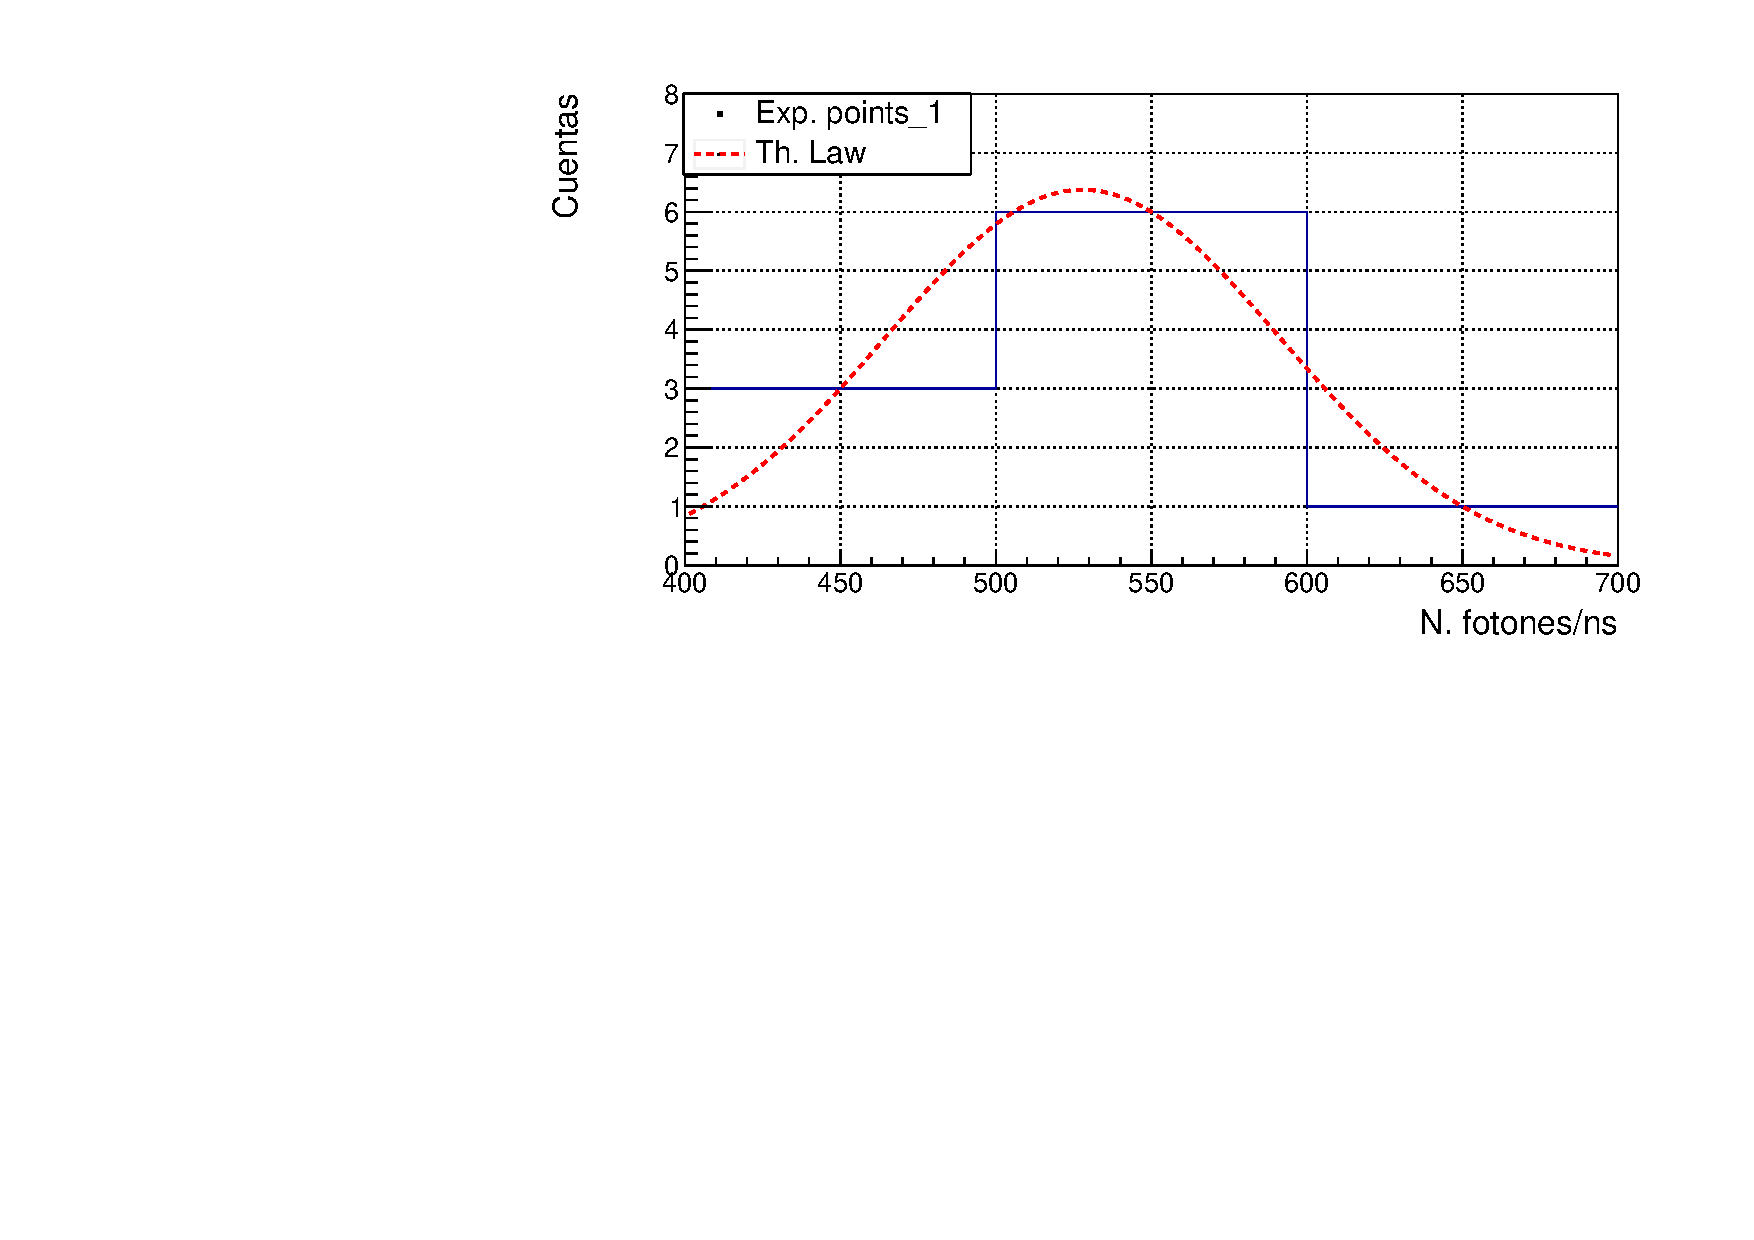
\includegraphics[scale=0.7]{Figuras/Nocladgauspos.pdf}
\caption{Histograma de las señales medidas para fibras no clad de 200 mm de longitud\label{posnoclad}}
\end{figure}

\begin{figure}[hbtp]
\centering
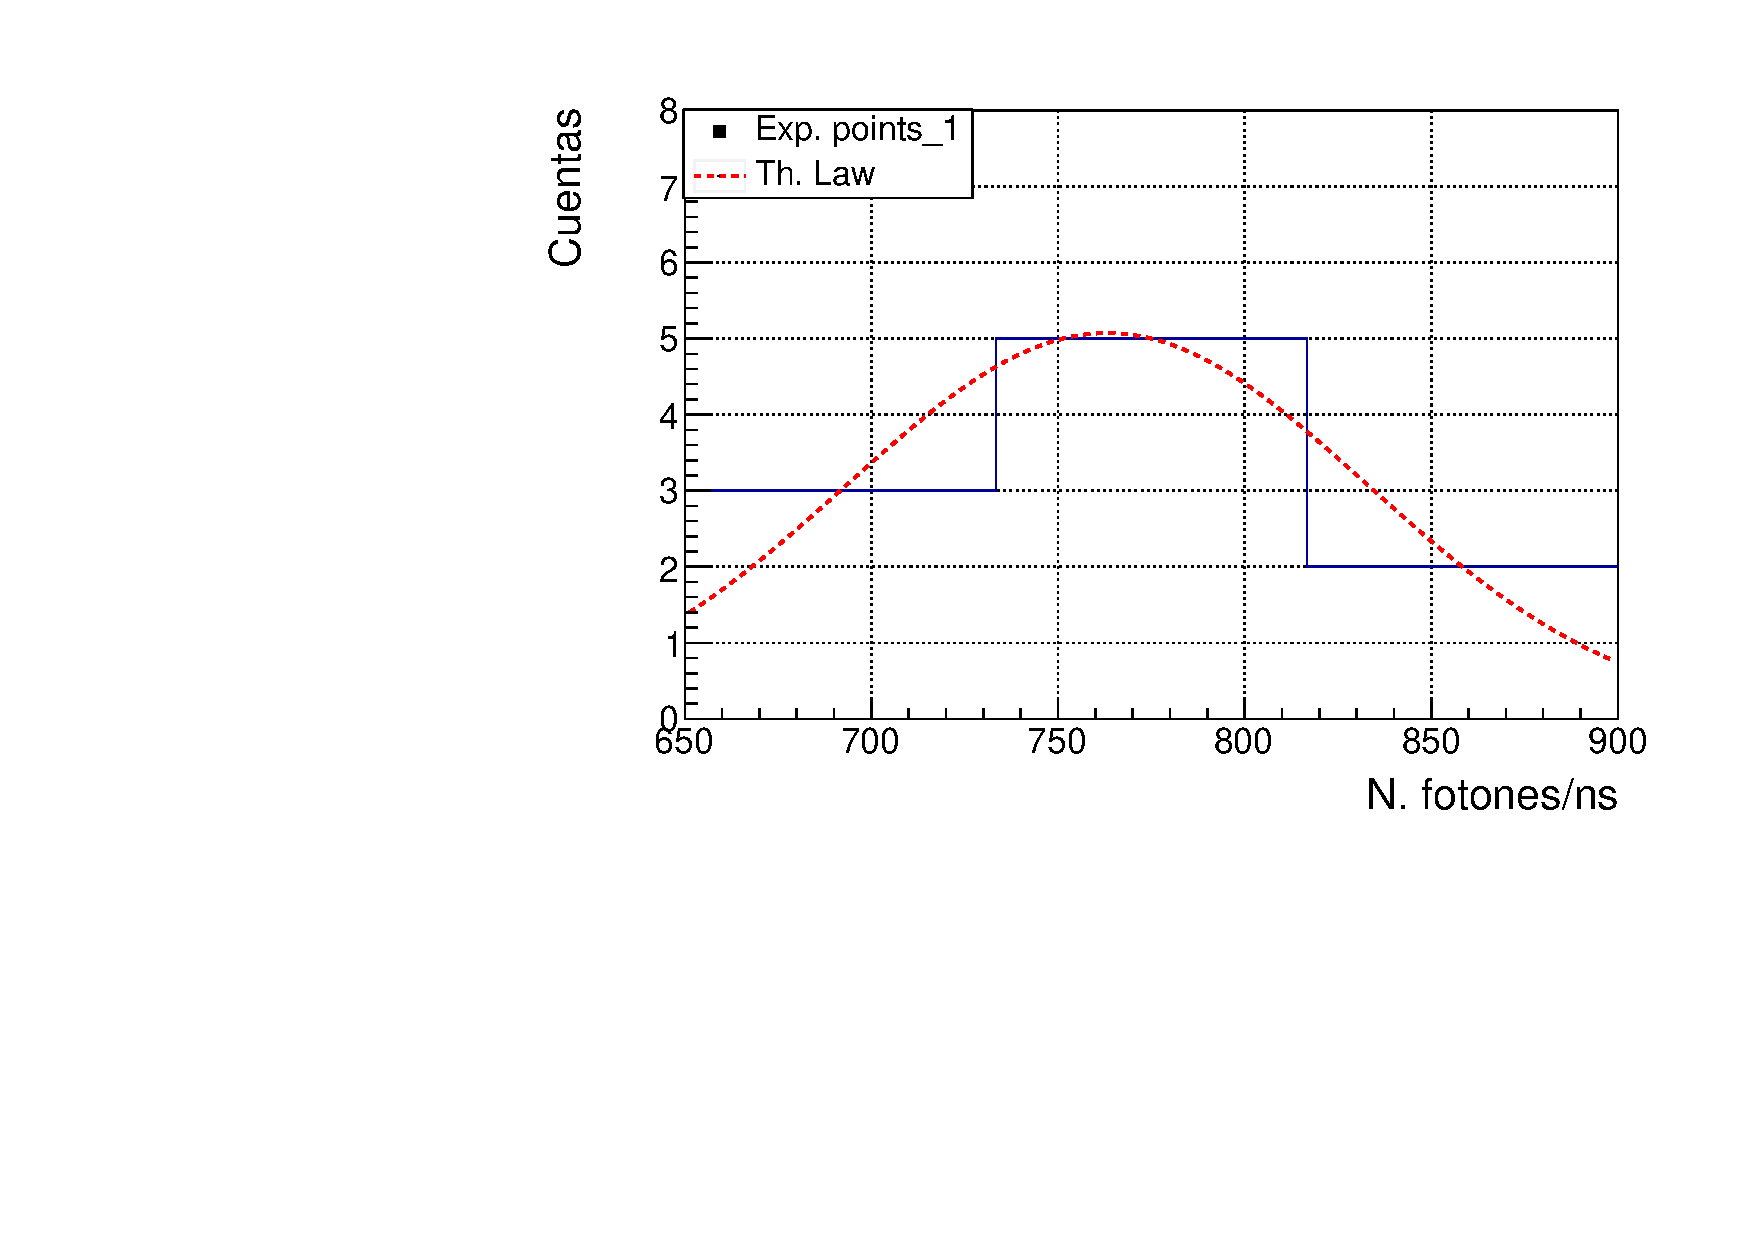
\includegraphics[scale=0.7]{Figuras/singlecladgauspos.pdf}
\caption{Histograma de las señales medidas para fibras single clad de 200 mm de longitud\label{possingleclad}}
\end{figure}

\begin{figure}[hbtp]
\centering
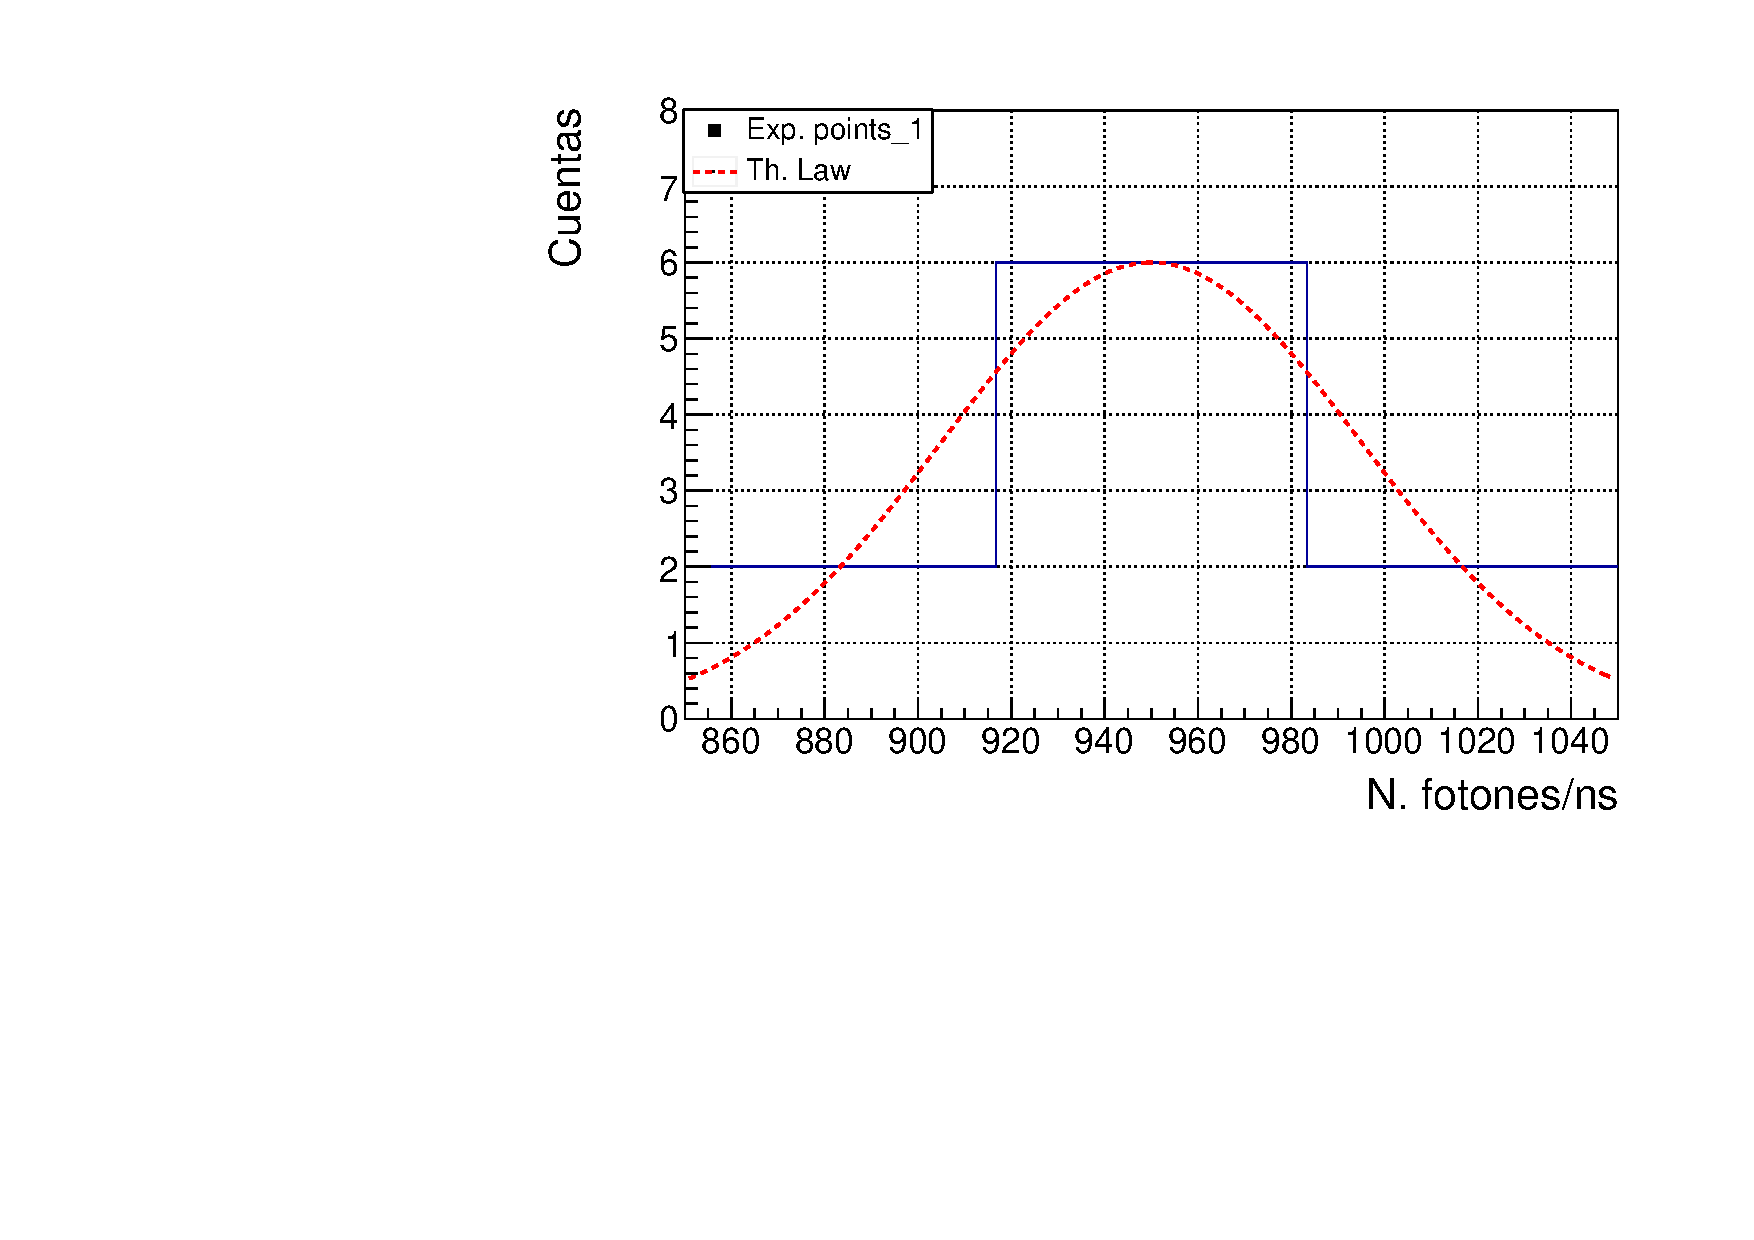
\includegraphics[scale=0.7]{Figuras/multicladgauspos.pdf}
\caption{Histograma de las señales medidas para fibras multi clad de 200 mm de longitud\label{posmulticlad}}
\end{figure}

Podemos observar que, como era de esperar, los resultados de cada experimento se distribuyen segun una gaussiana a la cual, se ha realizado un ajuste com opuede verse en las anteriores figuras \ref{posnoclad}, \ref{possingleclad} y \ref{posmulticlad}. Hay que tener en cuenta que, por el hecho de haber realizado el experimento para un número de repeticiones N relativamente bajo la resolución de esta gaussiana es mala.

Finalmente, para cada tipo de fibra, obtenemos la media y la desviación estandar según las expresiones \ref{ecuacionmedia} y \ref{ecuaciondesviacionestandar} respectivamente ya que este es un método más formal para un número de muestras N bajo:

\begin{equation}
\overline{x}=\sum_{i=1}^N \dfrac{x_i}{N}
\label{ecuacionmedia}
\end{equation}

\begin{equation}
\sigma=\dfrac{\sqrt{\sum_{i=1}^N (x_i-\overline{x})^2}}{N-1}
\label{ecuaciondesviacionestandar}
\end{equation}

Los valores obtenidos para cada tipo de fibra se muestran en la tabla \ref{tablasigmapos}

\begin{table}[H]
\begin{center}
\begin{tabular}{l | c | c | c | c }
Tipo de fibra & Media $(N.~\gamma/\nano\second)$ & Des. Std $(N.~\gamma/\nano\second)$ & Error $(N.~\gamma/\nano\second)$ & Des. Std. Rel\\
\hline \hline
No Clad & $524.09$ & $17.65$ & $0.010$ & $3.37$\\ 
Single clad & $765.63$ & $16.62$ & $0.012$ & $2.17$\\
Multi clad & $949.93$ & $9.91$ & $0.026$ & $1.04$\\
\end{tabular}
\caption{Resultado del estudio de la determinación de la desviación estandar debida a la posición de la fibra en el dispositivo experimental\label{tablasigmapos}}
\end{center}
\end{table}

En la tabla podemos observar que se a mostrado a demas una columna llamda "error". Este error es el obtenido por propagación del error aportado por el picoamperímetro en la medida, según se ha explicado antes. Los resultados que hemos sido capaces de determinar con este experimento son:

\begin{itemize}

\item{} Una medida del número de fotones por unidad de tiempo que cada tipo de fibra es capaz de recolectar para una misma intensidad de fotones a la entrada (la cual, si la conocemos, podríamos obtener la eficiencia absoluta de colección de luz de cada tipo de fibra). Podemos observar que esta recolección de luz es mayor a medida que aumenta el clad en la fibra, algo que cabría esperar ya que el principal objetivo de el clad es mejorar la colección de luz.

\item{} Una medida de la desviación estandar debida a la posición de la fibra en el dispositivo experimental para cada tipo de fibra, el cual era el objetivo inicial del estudio. Podemos observar que esta incertidumbre se mejora al añadir un primer cald y, esta mejora, se aumenta al añadir el segundo clad. Es decir, el cald no solo aporta una mejor recolección de luz, sino una mayor uniformidad en la señal obtenida ante lijeros desplazamientos de la fibra.

\item{} Se ha determinado por propagación el error experimental que asociado a la instrumentación empleada, el cual podemos observar que es tres órdenes de magnitud inferior a la desviación estandar, por lo que podemos despreciarlo en el estudio.

\item{} Finalmente se ha obtenido la desviación estandar relativa como el cociente entre la desviación estandar y la media. Podemos observar, como era de esperar, que este se reduce a medida que aumentamos el clad en la fibra.

\end{itemize}


%\newpage
\section{Medición de la desviación estandar debida al proceso de preparación de las fibras} \label{sec:sigmaint}
Ahora, con la desviación estandar debida a la posición de la fibra en el dispositivo experimental determianda, procedemos a llevar a cabo un estudio donde intervenga únicamente otra incertidumbre adicional, la debida a la preparación de cada una de las fibras utilizas.

Esta surje debido al hecho de que cada una de las fibras necesita de un proceso de preparación antes de poder estar ópticamente preparada para medir. Este proceso, como ya se ha comentado, incluye cortes con una guillotina especialmente diseñada en los talleres del IFIC, puido de las fibras con lijas de distinto grosor, limpieza de la superficie, etc. En resumen, se trata de un método individual para cada fibra que puede presentar cierta dispersión.

El estudio consistirá en preparar 10 muestras de $200~\mm$ diferentes para cada tipo de fibra y realizar la medida, con ayuda del picoamperímetro, de la intensidad promedio $I_i$ y su error para un conjunto de 100 medidas para cada una de estas fibras. Además, dado que solo pretendemos tomar una única medida en cada fibra, se realizará la medida para cuatro intensidades de alimentación de la LED diferentes, $0.05$, $0.1$, $0.15$ y $0.2~\milli\ampere$. De esta forma comprobaremos el correcto funcionamiento del sistema para cada uno de los casos al obtener una dependencia lineal.

El resultado de este experimento se representa en las figuras \ref{medidasnoclad}, \ref{medidassingleclad} y \ref{medidasmulticlad} 

\begin{figure}[hbtp]
\centering
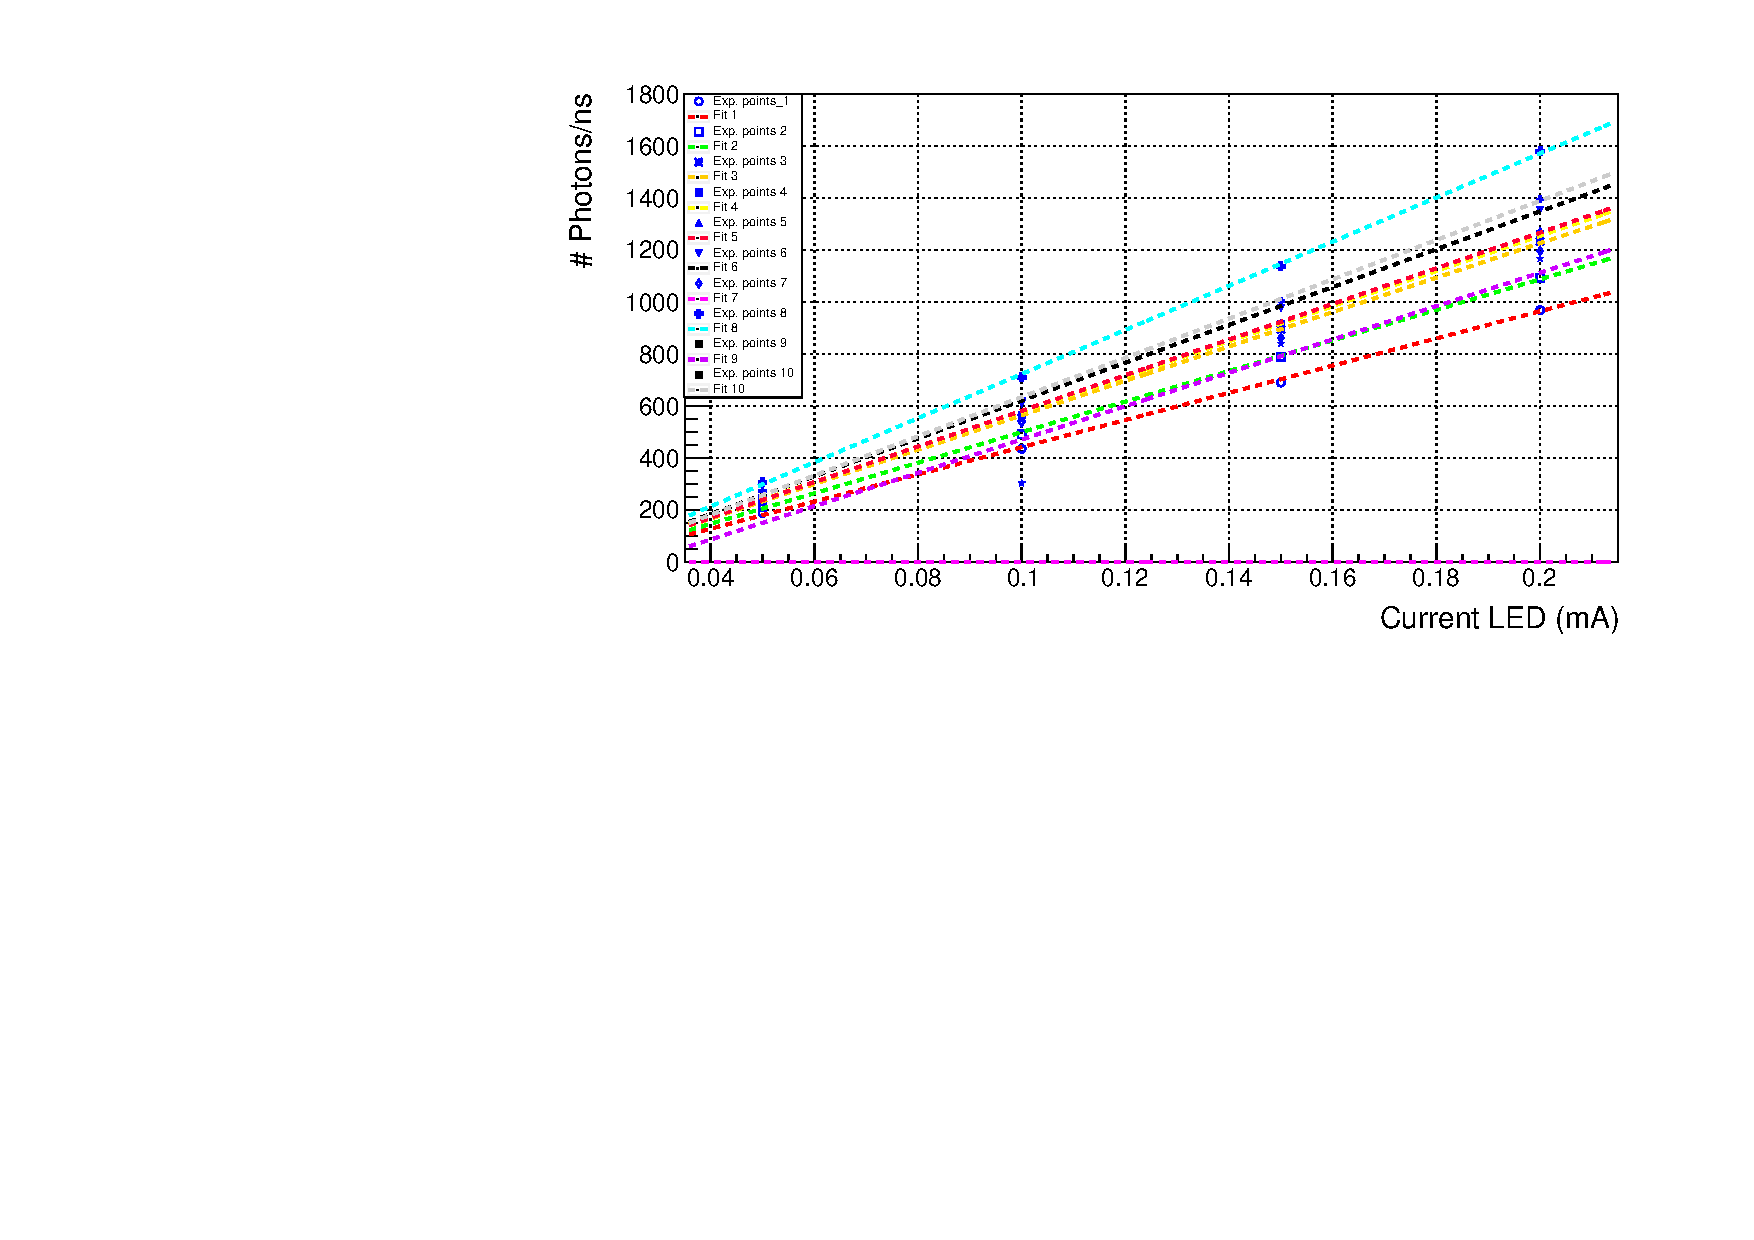
\includegraphics[scale=0.7]{Figuras/SamplesNoClad.pdf}
\caption{Intensidad obtenida en 10 muestras diferentes de fibras no clad de $200~\mm$ frente a la alimentaicón de la LED\label{medidasnoclad}}
\end{figure}

\begin{figure}[hbtp]
\centering
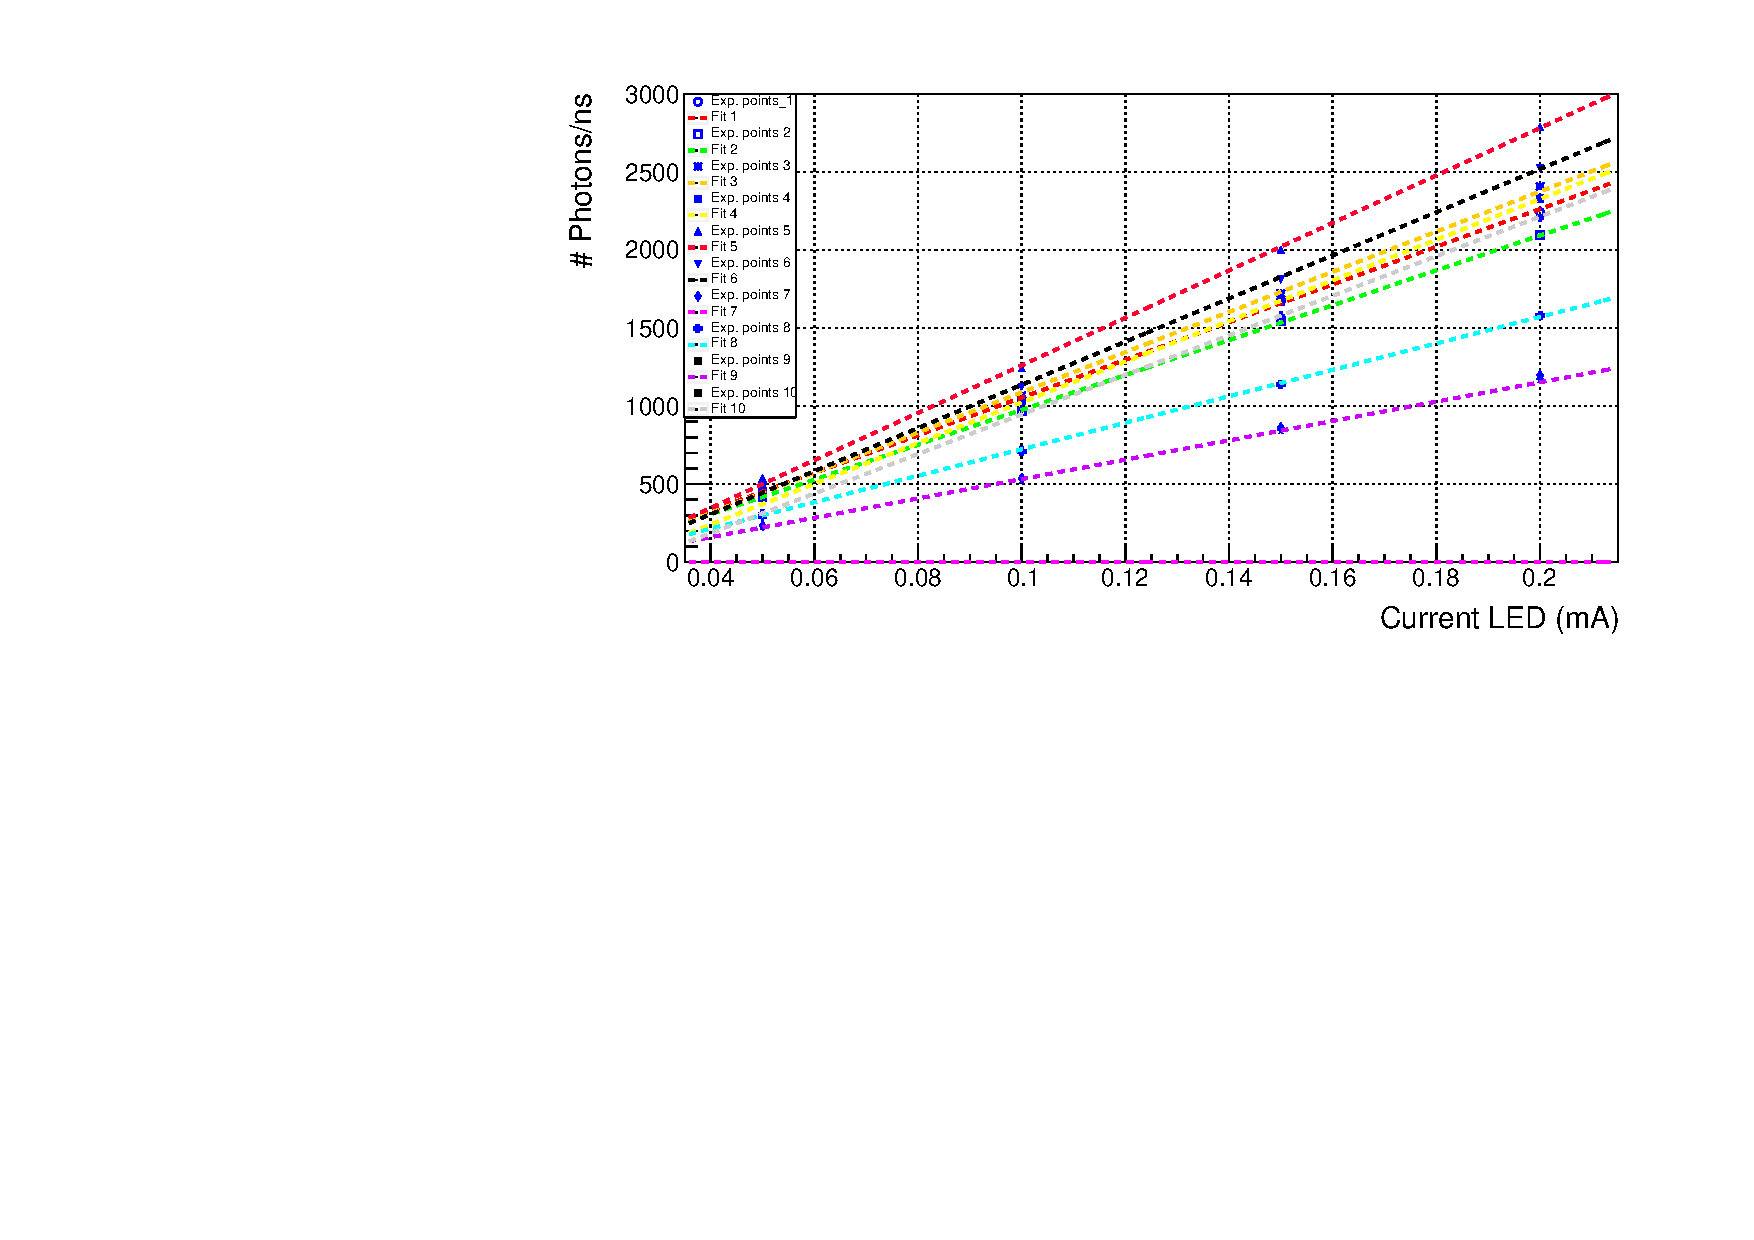
\includegraphics[scale=0.7]{Figuras/SamplesSingleCladHouda.pdf}
\caption{Intensidad obtenida en 10 muestras diferentes de fibras single clad de $200~\mm$ frente a la alimentaicón de la LED\label{medidassingleclad}}
\end{figure}

\begin{figure}[hbtp]
\centering
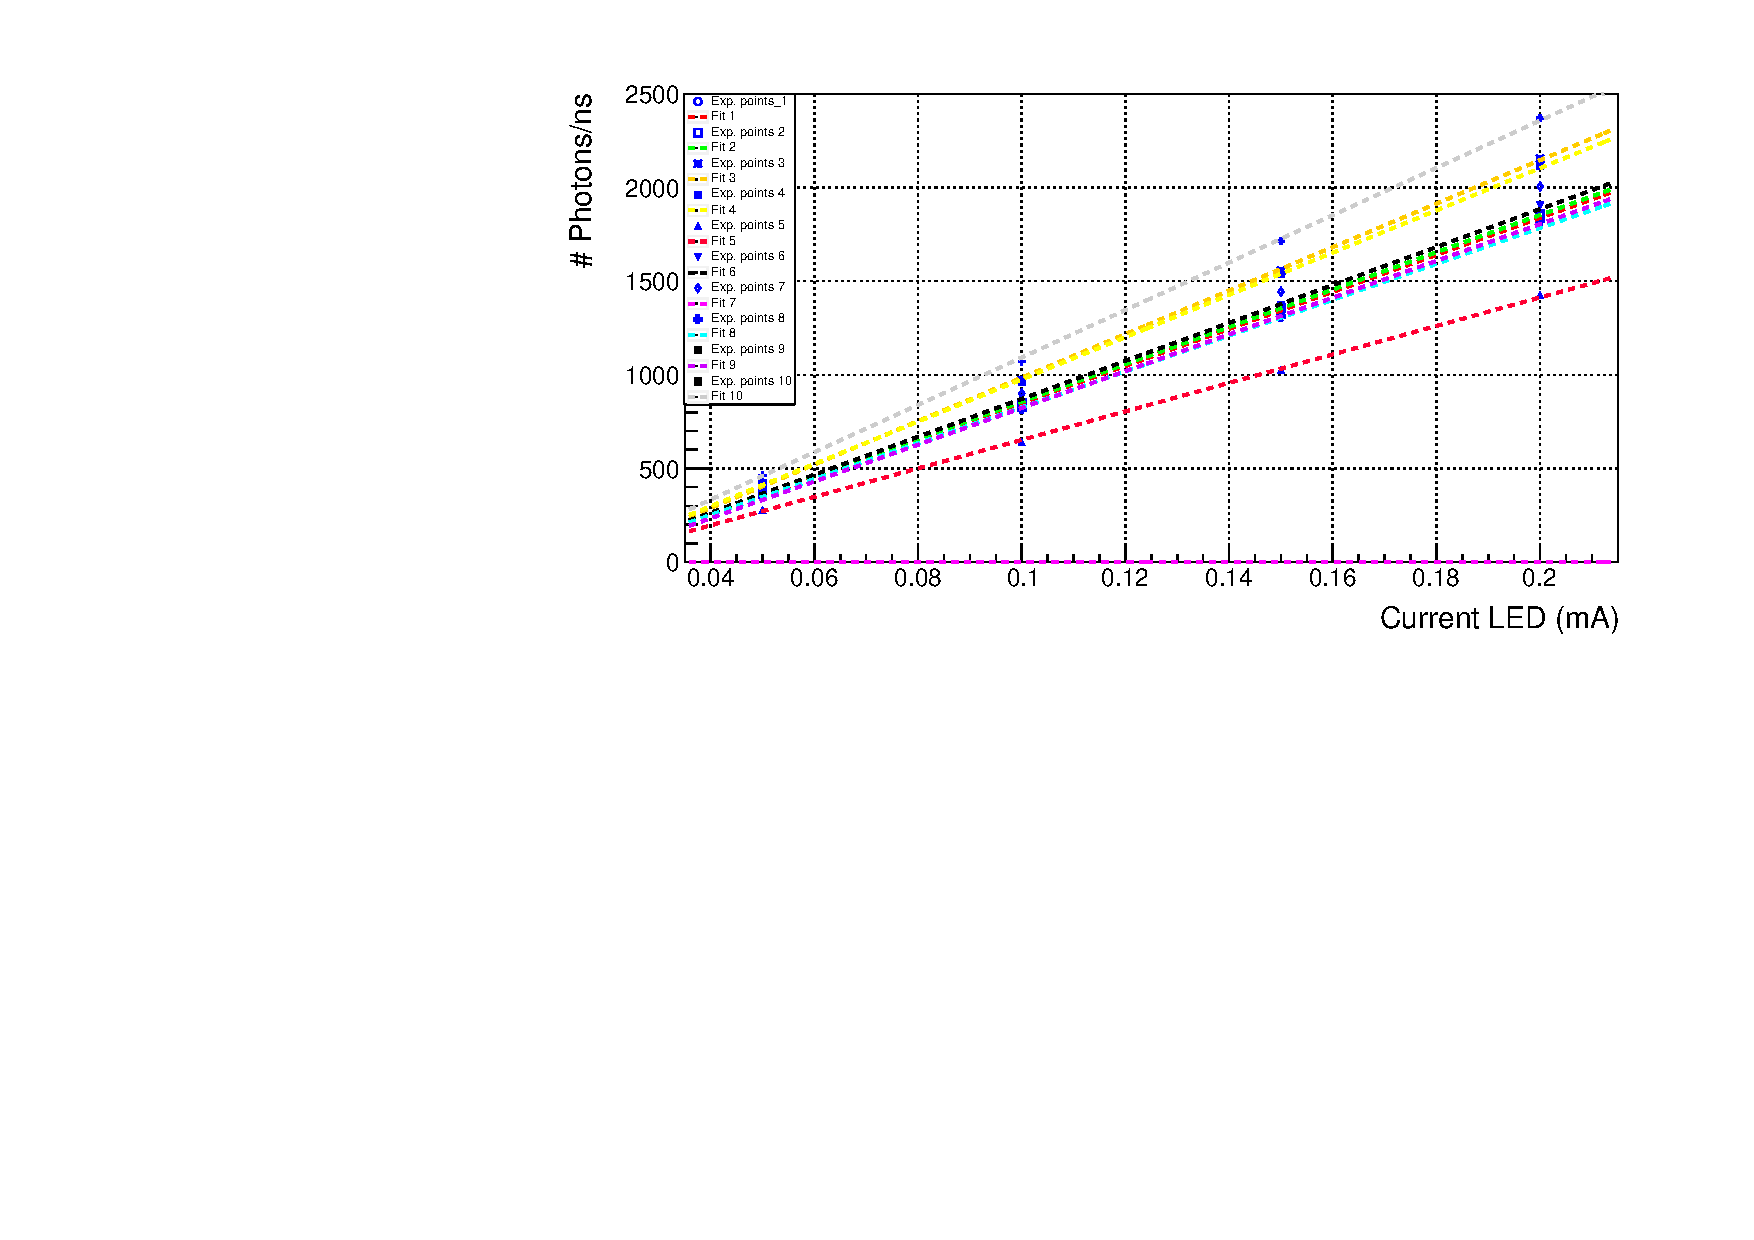
\includegraphics[scale=0.7]{Figuras/SamplesMultiClad.pdf}
\caption{Intensidad obtenida en 10 muestras diferentes de fibras multi clad de $200~\mm$ frente a la alimentaicón de la LED\label{medidasmulticlad}}
\end{figure}

En este podemos apreciar esta perfecta linealidad existente entre la señal y la alimentación de la LED para cada una de las muestras. También podemos observar que, efectivamente, existen diferencias entre la señal obtenidas con diferentes muestras de un mismot tipo de fibra. Ello es debido a dos razones, a la posición de la fibra en el dispostivo experimental y al proceso de preparación de la fibra. Por tanto, la desviación estandar total calculada en este experimento será la suma cuadrática de ambas según se expresa en la ecuación \ref{incertidumbreint}.

Con ayuda de las ecuaciones \ref{ecuacionmedia} y \ref{ecuaciondesviacionestandar}, obtenemos ahora el promedio de las diez medidas y la desviación estandar de estas para cada alimentación de la LED utilizada y cada tipo de fibra. El resultado puede verse en la tabla \ref{senalydesviacion}.

\begin{table}[H]
\begin{center}
\begin{tabular}{l | c | c | c | c }
Intensidad LED $(\milli\ampere)$ &  No Clad $(N.\gamma~/\nano\second)$ & Single Clad $(N.\gamma~/\nano\second)$ & Multi Clad $(N.\gamma~/\nano\second)$ \\
\hline \hline
$0.05$ & $243.46 \pm 9.82$ & $383.81 \pm 33.23$ & $376.676 \pm 14.96$\\ 
$0.1$ & $540.62 \pm 33.51$ & $922.68 \pm 73.97$ & $870.87 \pm 34.48$\\
$0.15$ & $902.74 \pm 36.83$ & $1485.10 \pm 119.90$ & $1396.60 \pm 55.24$\\
$0.2$ & $1252.62 \pm 50.48$ & $2053.78 \pm 166.391$ & $1932.57 \pm 76.02$\\

\end{tabular}
\caption{Señal y desviación estandar asociada a cada tipo de fibra y para cada alimetnación de la LED\label{senalydesviacion}}
\end{center}
\end{table}

Vemos que añadir un clad a la fibra produce una mejora considerable en la eficiencia de colección de luz. Sin embargo, para las distancias empleadas en el experimento, $200~\mm$, la mejora producida al añadir un segundo clad es inferior a las perdidas producidas por el hecho de tener que reducir el nucleo para ello, es decir, obtenemos una señal menor al aumentar el grosor del clad. Seguramente al aumentar de forma considerable la longitud de la fibra llegará un punto en el que esta situación cambie y la mejora producida por el doble clad sea superior a las perdidas producidas por la reducción del nucleo. Este sería un punto interesante y que se someterá a estudio en un futuro.

Hay que tener en cuenta que la señal obtenidas para el caso de fibras single clad esta en conflicto con la obtenidos en el apartado anterior. Tomaremos este valor como más fiable debido al hecho que este surje como promedio de 10 muestras distitnas de fibras mientras que el estudio anterior se ha realizado en todo momento sobre una misma muestra.

Ahora representamos estas tres dependencias promedidas en la figura \ref{mediafibras}:

\begin{figure}[H]
\centering
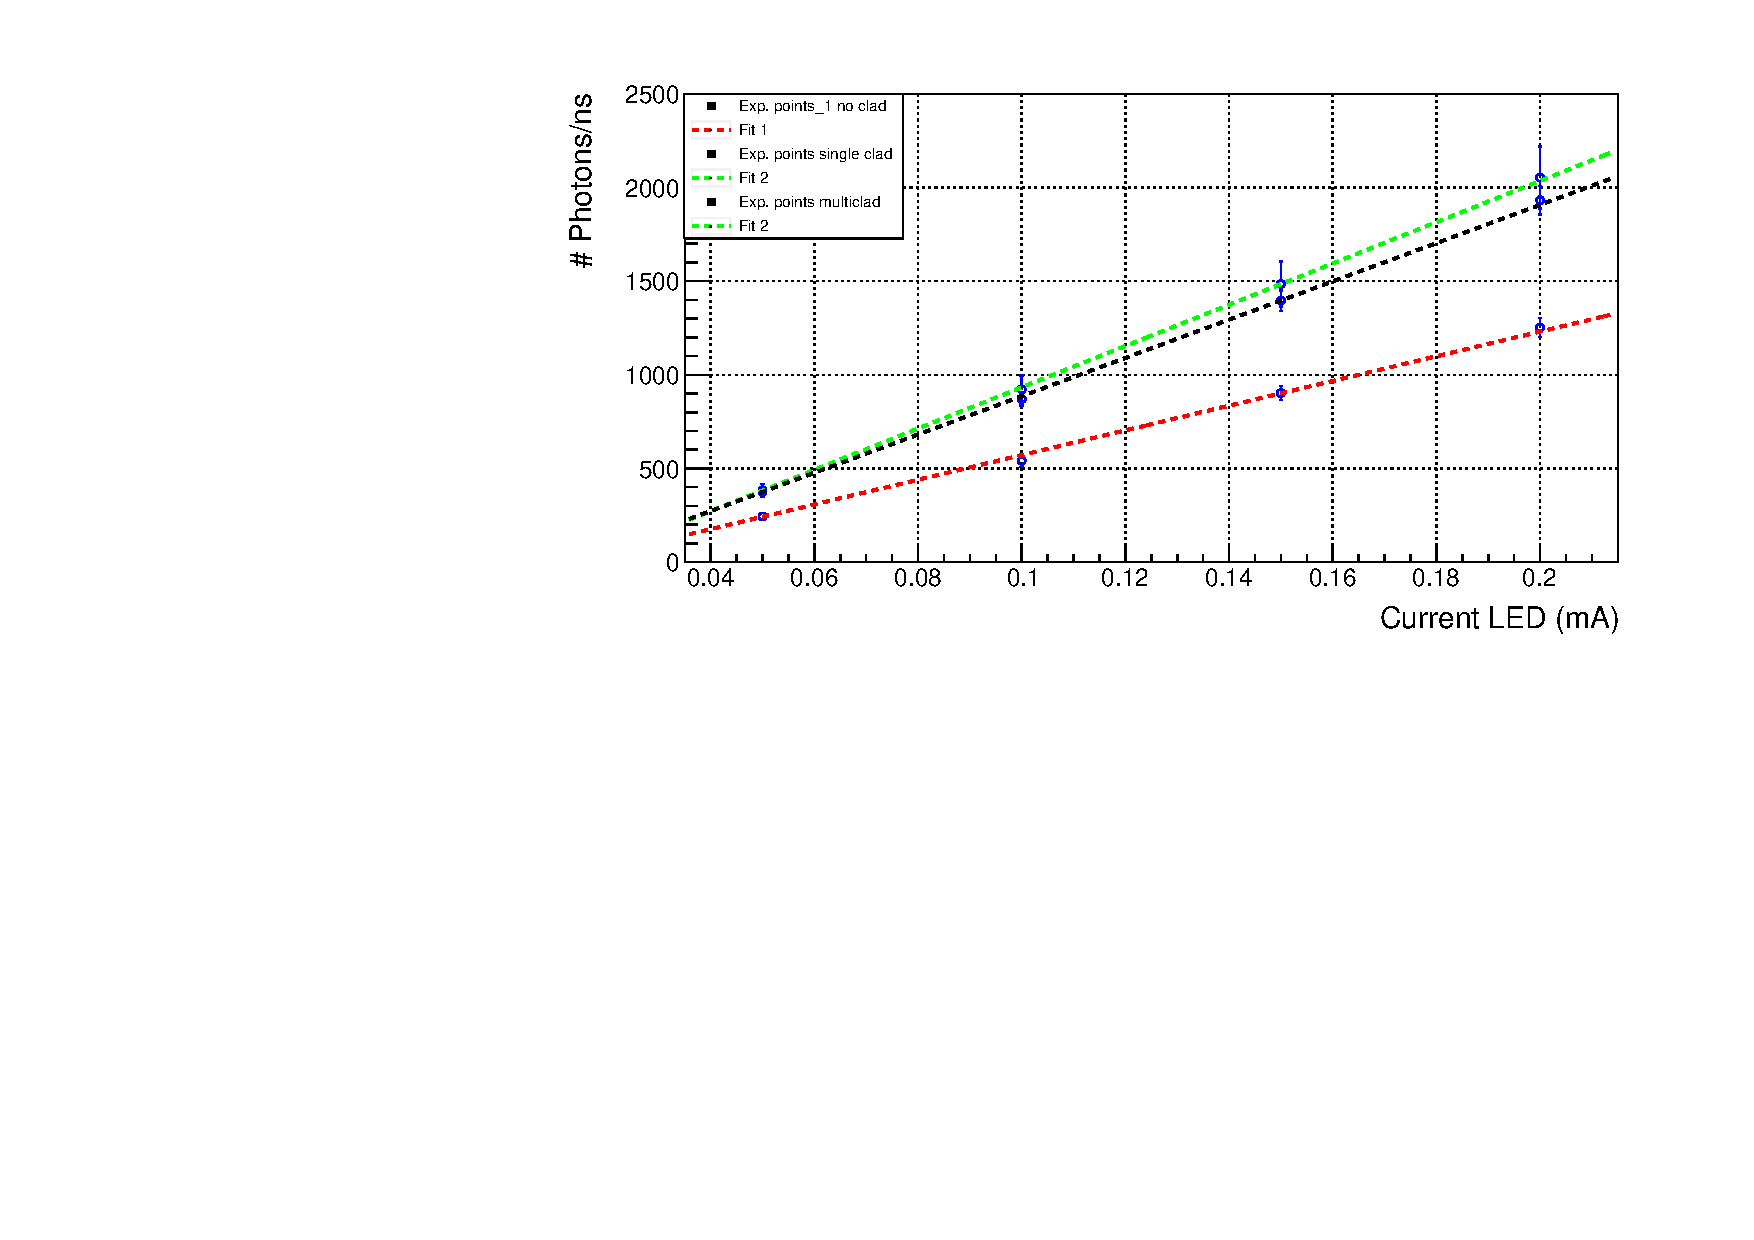
\includegraphics[scale=0.7]{Figuras/HoudaCase.pdf}
\caption{Media y desviación estandar de las 10 muestras de fibras de cada tipo de $200~\mm$ frente a la alimentaicón de la LED\label{mediafibras}}
\end{figure}


Además de lo comentado anteriormente, podemos observar una relación perfecta mente lineal para cada uno de los tipos lo cual nos permite verificar que el estudio se ha realizado adecuadamente.

Finalmente obtenemos la dispersión estandar relativa como el cociente entre la dispersión estandar y la señal. Realizamos este para cada una de las cuatro intensidades de alimentación de la LED y, dado que teóricamente este debería de ser constante, obtenemos el promedio. Los resultados pueden observarse en la tabla \ref{relativefibers}:

\begin{table}[H]
\begin{center}
\begin{tabular}{l | c | c | c | c }

Intensidad LED $(\milli\ampere)$ & D. S. R. (No Clad) & D. S. R. (Single Clad) & D. S. R. (Multi Clad)\\
\hline \hline
0.05 & $4.03$ & $8.66$ & $3.97$\\ 
0.1 & $6.20$ & $8.02$ & $3.91$\\
0.15 & $4.08$ & $8.04$ & $3.96$\\
0.2 & $4.03$ & $8.10$ & $3.93$\\
\hline \hline
Averege & $4.59\pm 0.54$ & $8.21\pm0.15$ & $3.96 \pm 0.01$

\end{tabular}
\caption{Desviación estandar relativa asociada a cada tipo de fibra y para cada alimetnación de la LED\label{relativefibers}}
\end{center}
\end{table}

Estos valores corresponden a la desviación estandar relativa total para cada una de las tres fibras. Ahora, con ayuda de la ecuación \ref{incertidumbreint}, es inmediato obtener el valor de la incertidumbre relativa asociada al proceso de fabricación. Un resumen de esto se muestra en la tabla \ref{incertidumbres}

\begin{table}[H]
\begin{center}
\begin{tabular}{l | c | c | c | c }
Type of fiber & $\sigma_{total,rel}$ (\%) & $\sigma_{pos,rel}$ (\%) &$\sigma_{int,rel}$ (\%)\\
\hline \hline
No Clad & 4.58 +- 0.53 & 3.37 & 3.10\\ 
Single Clad & 8.21 +- 0.15 & 2.17 & 7.92\\
Multi Clad & 3.96 +- 0.01 & 1.04 & 3.82
\end{tabular}
\caption{Resumen de las incertidumbres obtenidas en el estudio de las fibras\label{incertidumbres}}
\end{center}
\end{table}

Podemos observar que, la mínima incertidumbre en el proceso de preparación de la fibra se encuentra en la fibra sin clad, es decir, el elemento de la fibra más resistente a este proceso es el nucleo. Podemos observar que, al añadirle un clad simple esta incertidumbre se dispara. El motivo de ello es que el clad, por el hecho de ser tan fino, se estropea con facilidad en el proceso de preparación, un proceso relativamente agresivo, algo que puede llegarse a observar incluso a simple vista. Sin embargo, podemos observar que, el hecho de añadir un segundo clad mejora notablemente la incertidumbre. Es decir, este segundo clad no solo aporta una lijera mejora en al eficiencia de colección de luz, si no que aporta una mayor robustez a la fibra. 

%\newpage
\section{Implementación de un exhaustivo protocolo de limpieza de la superficie de las fibras} \label{sec:liempieza}
A continuación procedemos a cuantificar la importancia de la limpieza de la superficie de las fibras. El motivo de ello es que, para el proyecto Tritium, que utiliza fibras sin clad, el estado de la superficie es muy impotante ya que esta \textit{interface} formada entre el clad y el agua tritiada será la que marcará la mayor o menor tasa de conservación de los fotones. Lo mismo ocurrirá para fibras con single clad o multi clad, pero de forma menos importante.

La forma con la que pretendemos cuantificar la importancia del tratamiento de las superficies de las fibras será repetir la sección \ref{sec:sigmaint} pero, en cada fibra sometida a estudio, se incluirá una exhaustiva tarea de limpieza con ayuda de alcohol 2-isopropanol. Unicamente se realizará para un tipo de fibra, single clad, debido al tiempo que se necesita para llevar a cabo esta tarea. Se realizará sobre el tipo single clad ya que, en esta, se encontró una confrotación de los resultados obtenidos para la señal entre dos estudios anteriores.

Por tanto, preparamos 10 muestras diferentes de fibras single clad de $20~\cm$ y, con ayuda de alcohol y unos pañuelos especialmente preparados para su utilización en salas blancas, realizamos una exhaustiva limpieza sobre la superficie de cada fibra.

De forma análoga a la sección \ref{sec:sigmaint} mostramos a continuación los resultados del experimento:

\begin{figure}[hbtp]
\centering
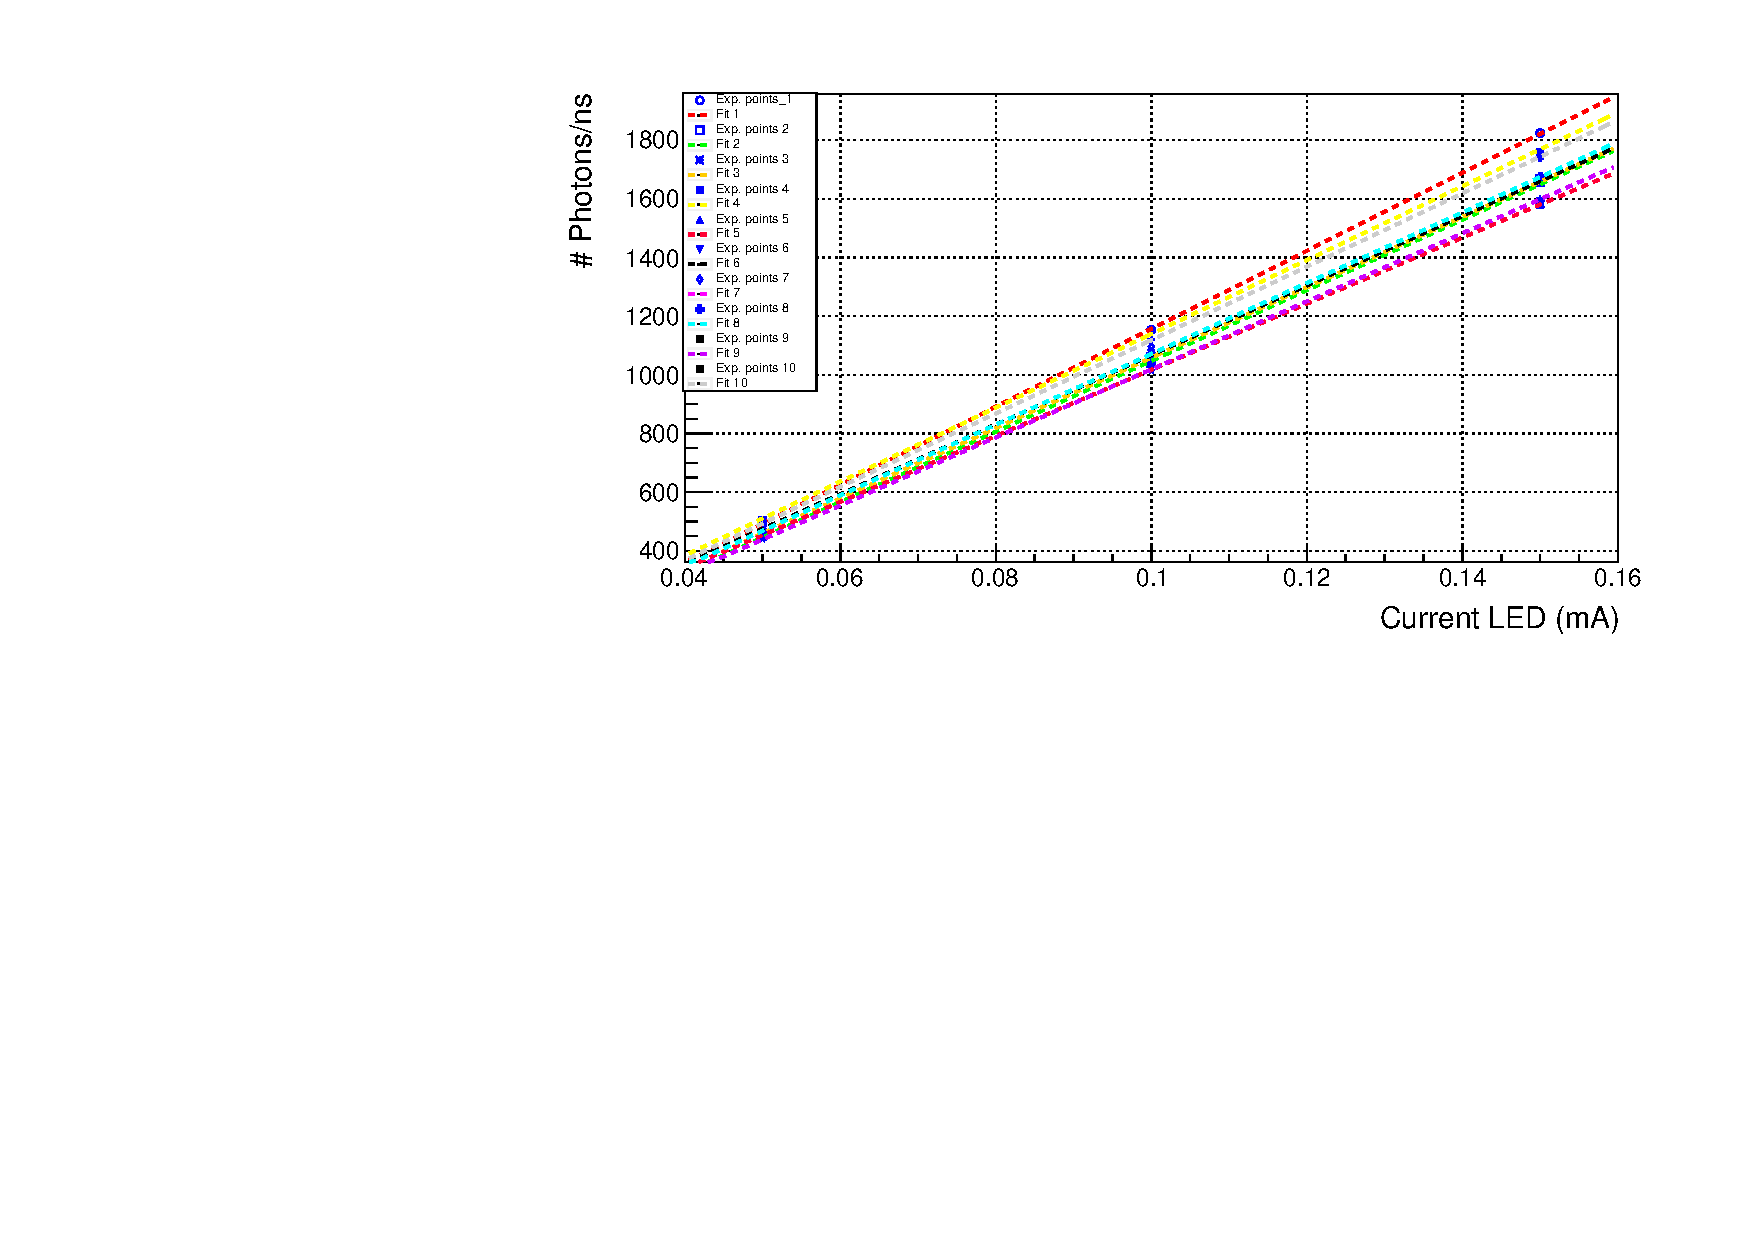
\includegraphics[scale=0.7]{Figuras/SamplesSingleCladMarcos.pdf}
\caption{Intensidad obtenida en 10 muestras diferentes de fibras single clad de $200~\mm$ frente a la alimentaicón de la LED con la implementación del tratamiento de superficie\label{medidassinglecladlimpieza}}
\end{figure}

De nuevo observamos una perfecta linealidad de la señal en cada una de las fibras frente a la alimentación de la LED. Con ayuda de las expresiones \ref{ecuacionmedia} y \ref{ecuaciondesviacionestandar} obtenemos su promedio y desviación estandar. Los resultados se muestran en la tabla \ref{singlecladlimpieza}, donde se incluyen los resultados anteriores obtenidos sin la implementación de este tratamiento de las superficies:

\begin{table}[H]
\begin{center}
\begin{tabular}{l | c | c | c | c }
Intensidad LED $(\milli\ampere)$ &  Sin tratamiento $(N.\gamma~/\nano\second)$ & Con tratamiento $(N.\gamma~/\nano\second)$ \\
\hline \hline
$0.05$ & $383.81 \pm 33.23$ & $470.60 \pm 6.57$\\ 
$0.1$ & $922.68 \pm 73.97$ & $1082.28 \pm 14.27$\\
$0.15$ & $1485.10 \pm 119.90$ & $1681.65 \pm 24.82$\\
$0.2$ & $2053.78 \pm 166.391$ & $ --- $\\

\end{tabular}
\caption{Señal y desviación estandar para fibras single clad con y sin tratamiento de la superficie para cada alimetnación de la LED\label{singlecladlimpieza}}
\end{center}
\end{table}

Podemos notar la sutileza que ahora no se ha llegado a medir el caso de $0.2~\milli\ampere$. El motivo de ello fueron una serie de complicaciones técnicas. Sin embargo, debido a la alta linealidad de la respuesta del sistema, podemos considerar que estas complicaciones no afectarán de forma significativa al resultado del experimento. Seguidamente resumimos esta tabla en un gráfico donde se muestran ambas señales superpuestas: 

\begin{figure}[hbtp]
\centering
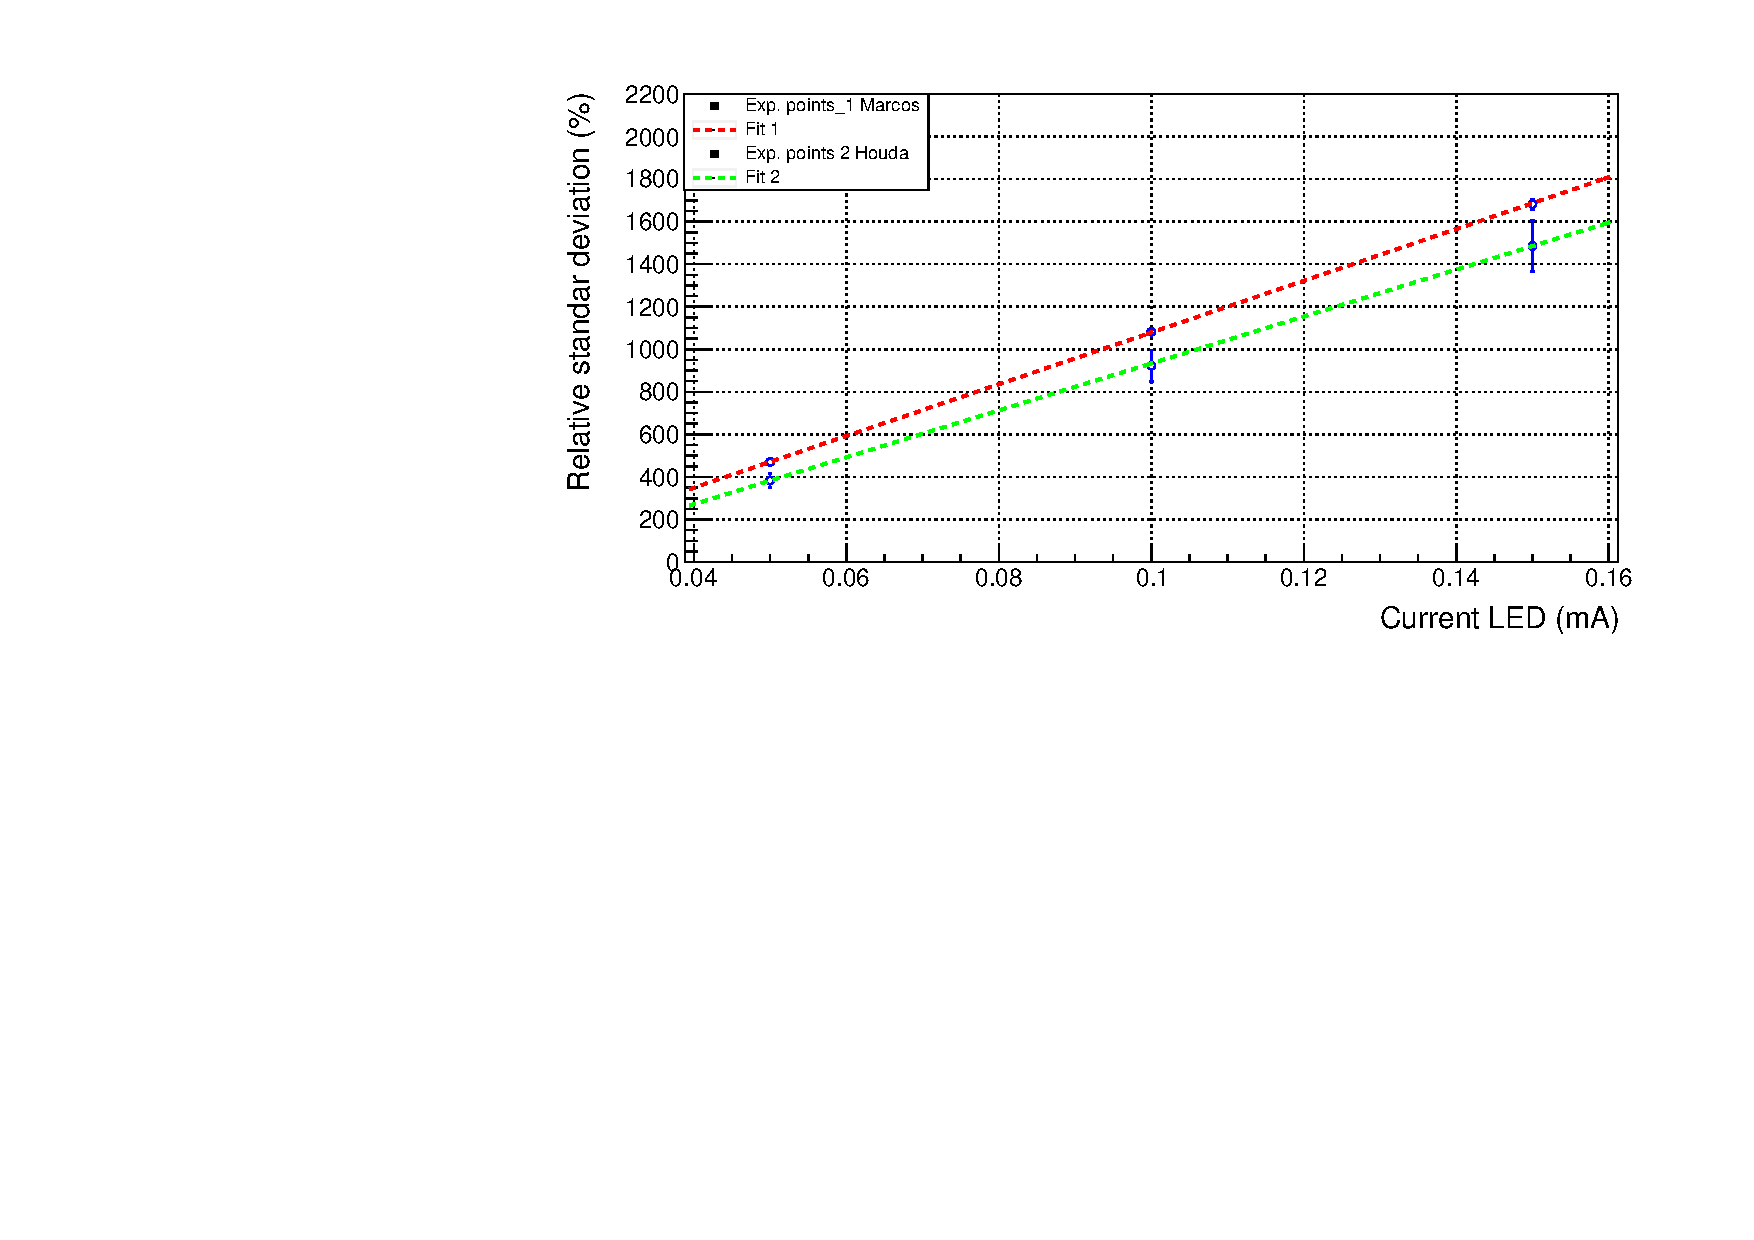
\includegraphics[scale=0.7]{Figuras/comparacion.pdf}
\caption{Intensidad promediada de 10 muestras diferentes de fibras single clad de $200~\mm$ frente a la alimentaicón de la LED con y sin la implementación del tratamiento de superficie\label{promediosinglecladlimpieza}}
\end{figure}

Podemos observar, en primer lugar, un lijero aumento de la señal obtenida con dichas fibras. La razon de ello es, como ya se ha explicado, una mejora de la eficiencia de recolección. En segundo lugar, podemos apreciar una considerable reducción  de las incertidumbres asociadas a cada uno de los promedios, algo realmente importante desde el punto de vista del proyecto Tritium ya que este busca trabajar con un número considerable de fibras. 

En último lugar incluimos la tabla \ref{comparacionincertidumbres} donde se presentan las distintas desviaciones estandar relativas obtenidas en cada caso:

\begin{table}[H]
\begin{center}
\begin{tabular}{l | c | c | c | c }
Person & $\sigma_{total} (\%) $ & $\sigma_{pos} (\%)$\\
\hline \hline
Con tratamiento & 1.4  & 2.17\\ 
Sin tratamiento & 8.2 & 2.17\\
\end{tabular}
\caption{Desviaciones estandar relativas obtenidas para cada caso\label{comparacionincertidumbres}}
\end{center}
\end{table}

En primer lugar podemos ver que se ha verificado la confrotación de resultados en la señal debida al caso single clad. Además, en segundo lugar, podemos observar que, con la implementación de un exhaustivo método de tratamiento de la superficie previo al momento de la realización de la medida se ha conseguido disminuir la incertidumbre hasta en un $82.93\%$, factor muy importante y de gran implicación en el proyecto Tritium. De hecho, su reducción fue tal que imposibilito la obtención de la desviación estandar debida al proceso de preparación de las fibras, el cual lo obtenemos con ayuda de la ecuación \ref{incertidumbreint}, por el simple hecho que obtenemos un valor negativo en el interior de la raiz. 

Debido a ello necesitamos recalcular la desviación estandar asociada a la posición de la fibra en el SetUp con la implementación de este proceso de tratamiento de la superficie. De manera totalmente análoga a la sección \ref{sec:sigmapos} presentamos los resultados en el siguiente histograma:

\begin{figure}[hbtp]
\centering
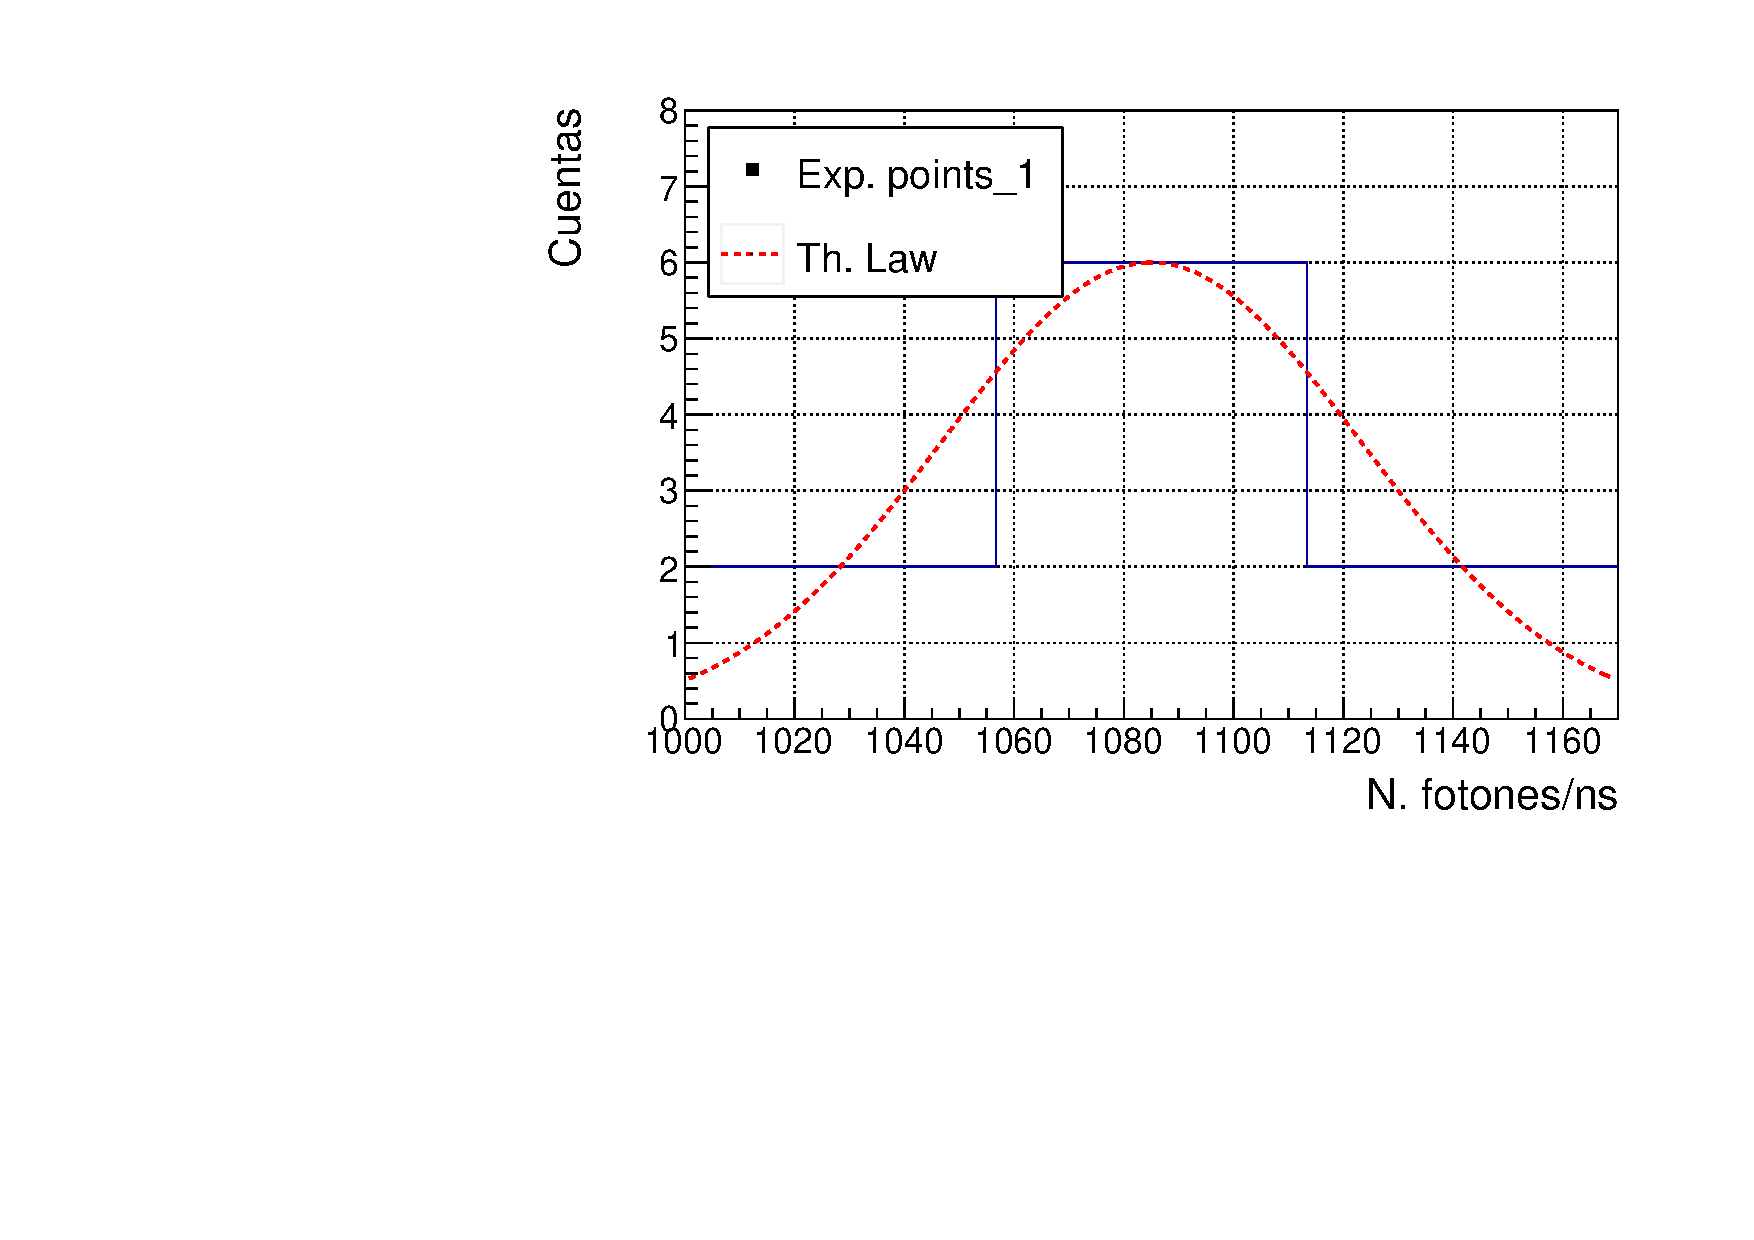
\includegraphics[scale=0.7]{Figuras/singlecladsigmaposgausclean.pdf}
\caption{Intensidad promediada de 10 muestras diferentes de fibras single clad de $200~\mm$ frente a la alimentaicón de la LED con y sin la implementación del tratamiento de superficie\label{promediosinglecladlimpieza}}
\end{figure}

Donde, con ayuda de las ecuaciones \ref{ecuacionmedia} y \ref{ecuaciondesviacionestandar}, obtenemos un resultado de $S=1071.70~\pm~9.07~N. \gamma/\nano\second$, resultado que, de nuevo, confirma la confrotación entre resultados que obtuvimos en el pasado.

 Podemos observar que se ha obtenido un valor para la desviación estandar relativa de $0.85\%$, valor considerablemente menor que el caso anterior. Por tanto vemos que, con la implementación del tratamiento de la superficie conseguimos una reducción de la incertidumbre asociada a la posición de hasta un $61\%$, valor que nos confirma nuevamente que el método de tratamiento de la superficie de la fibra funciona.
 
Finalmente, con ayuda de este valor y de la ecuación \ref{incertidumbreint}, obtenemos la desviación estandar debida únicamente al proceso de preparación de las fibras. Este resultado, junto con el caso anterior sin tratamiento, se muestra en la tabla \ref{resultadofinalclean}:

\begin{table}[H]
\begin{center}
\begin{tabular}{l | c | c | c | c }
Person & $\sigma_{total} (\%) $ & $\sigma_{pos} (\%)$ & $\sigma_{int} (\%)$\\
\hline \hline
Con tratamiento & 1.4  & 0.85 & 1.11\\ 
Sin tratamiento & 8.2 & 2.17 & 7.91\\
\end{tabular}
\caption{Desviaciones estandar relativas obtenidas para cada caso\label{resultadofinalclean}}
\end{center}
\end{table}

Vemos por tanto que ha quedado demostrada la notable disminución de la desviación standar de la señal asociada a la fibras al incluir en su protocolo de preparación un tratamiento para las superficies. Debido a ello, en la construcción del prototipo Tritium 1, se desarrolló e incluyo un método de tratamiento de las superficies de cada una de las fibras que se utilizó. Este método se explica en la sección \ref{sec:limpiezaICMOL}.

%\newpage
\section{Implementación de un exhaustivo protocolo de limpieza de la superficie de las fibras para la construcción del prototipo Tritium 1} \label{sec:limpiezaICMOL}
\input{./Secciones/LimpiezaICMOL}

%\newpage
\section{Comprobación de la necesidad de pulir ambas secciones de la fibra en el prototipo Tritium 1} \label{sec:ambascaras}
Finalmente, llegados a este punto, se procedío a quantificar hasta que punto es necesario realizar el pulido de ambas superficies transversales de la fibra. Este estudio esta enfocado al hecho que el prototipo Tritium 1, a diferencia del prototipo Tritium 0, únicamente realiza la lectura por una de las dos superficies de cada fibra. El motivo de ello es que, por un lado, se observó la necesidad de imponer una configuración rectilinea en el detector para mejorar su eficiencia de recolección y, en segundo lugar, se tuvieron en cuenta una serie de  equerimientos debidos a seguridad nuclear. 

Debido al hecho de que el prototipo Tritium 1 únicamente mide por un lado y su lado contrario se encuentra totalmente recubierto de teflón, estudiamos la necesidad de pulir ambas caras ya que se trata de un proceso duro y largo. Para ello utilizamos el dispositivo experimental mostrado en la imagen \ref{setupcaras}.

\begin{figure}[hbtp]
\centering
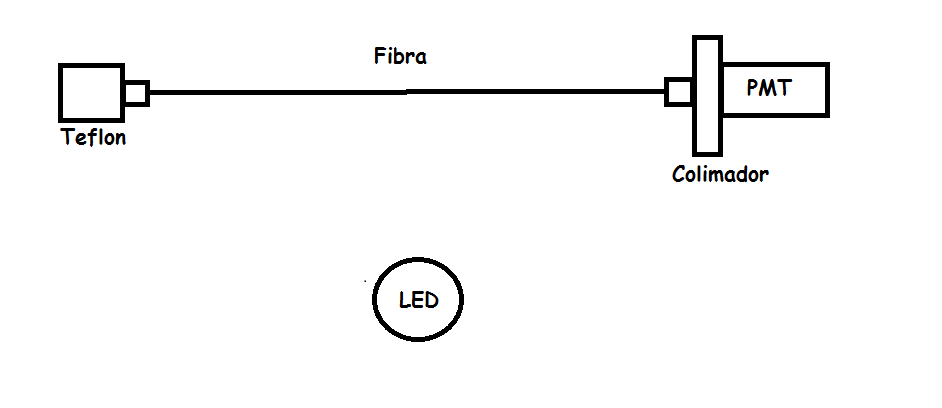
\includegraphics[scale=0.7]{Figuras/SetUpLED.png}
\caption{Dispositivo experimental utilizado para llevar a cabo el estudio.\label{setupcaras}}
\end{figure}

Este consiste en el mismo dispositivo empleado en el estudio anterior pero en el que la LED se ha desplazado a una posición para realizar una incidencia lateral de los fotones. Finalmente, un extremo de la fibra se encuentra totalmente recubierto de teflon y realizamos la lectura de la señal por el otro lado (simulando la situación del detector). Las fibras empleadas fueron de tipo single clad de $200~\mm$ de longitud ya que son las empleadas en el proyecto Tritium.

En primer lugar se realizo este experimento para tres muestras diferentes de fibras en las que solo se había pulido el extremo por el que se realizaba la lectura. En segundo lugar se repitió este mismo experimento con las mismas muestras a las que, además, se les había realizado un segundo pulido en el otro extremo.

Ambos resultados pormediados se muestran en la figura \ref{resultadoscaras}.

\begin{figure}[hbtp]
\centering
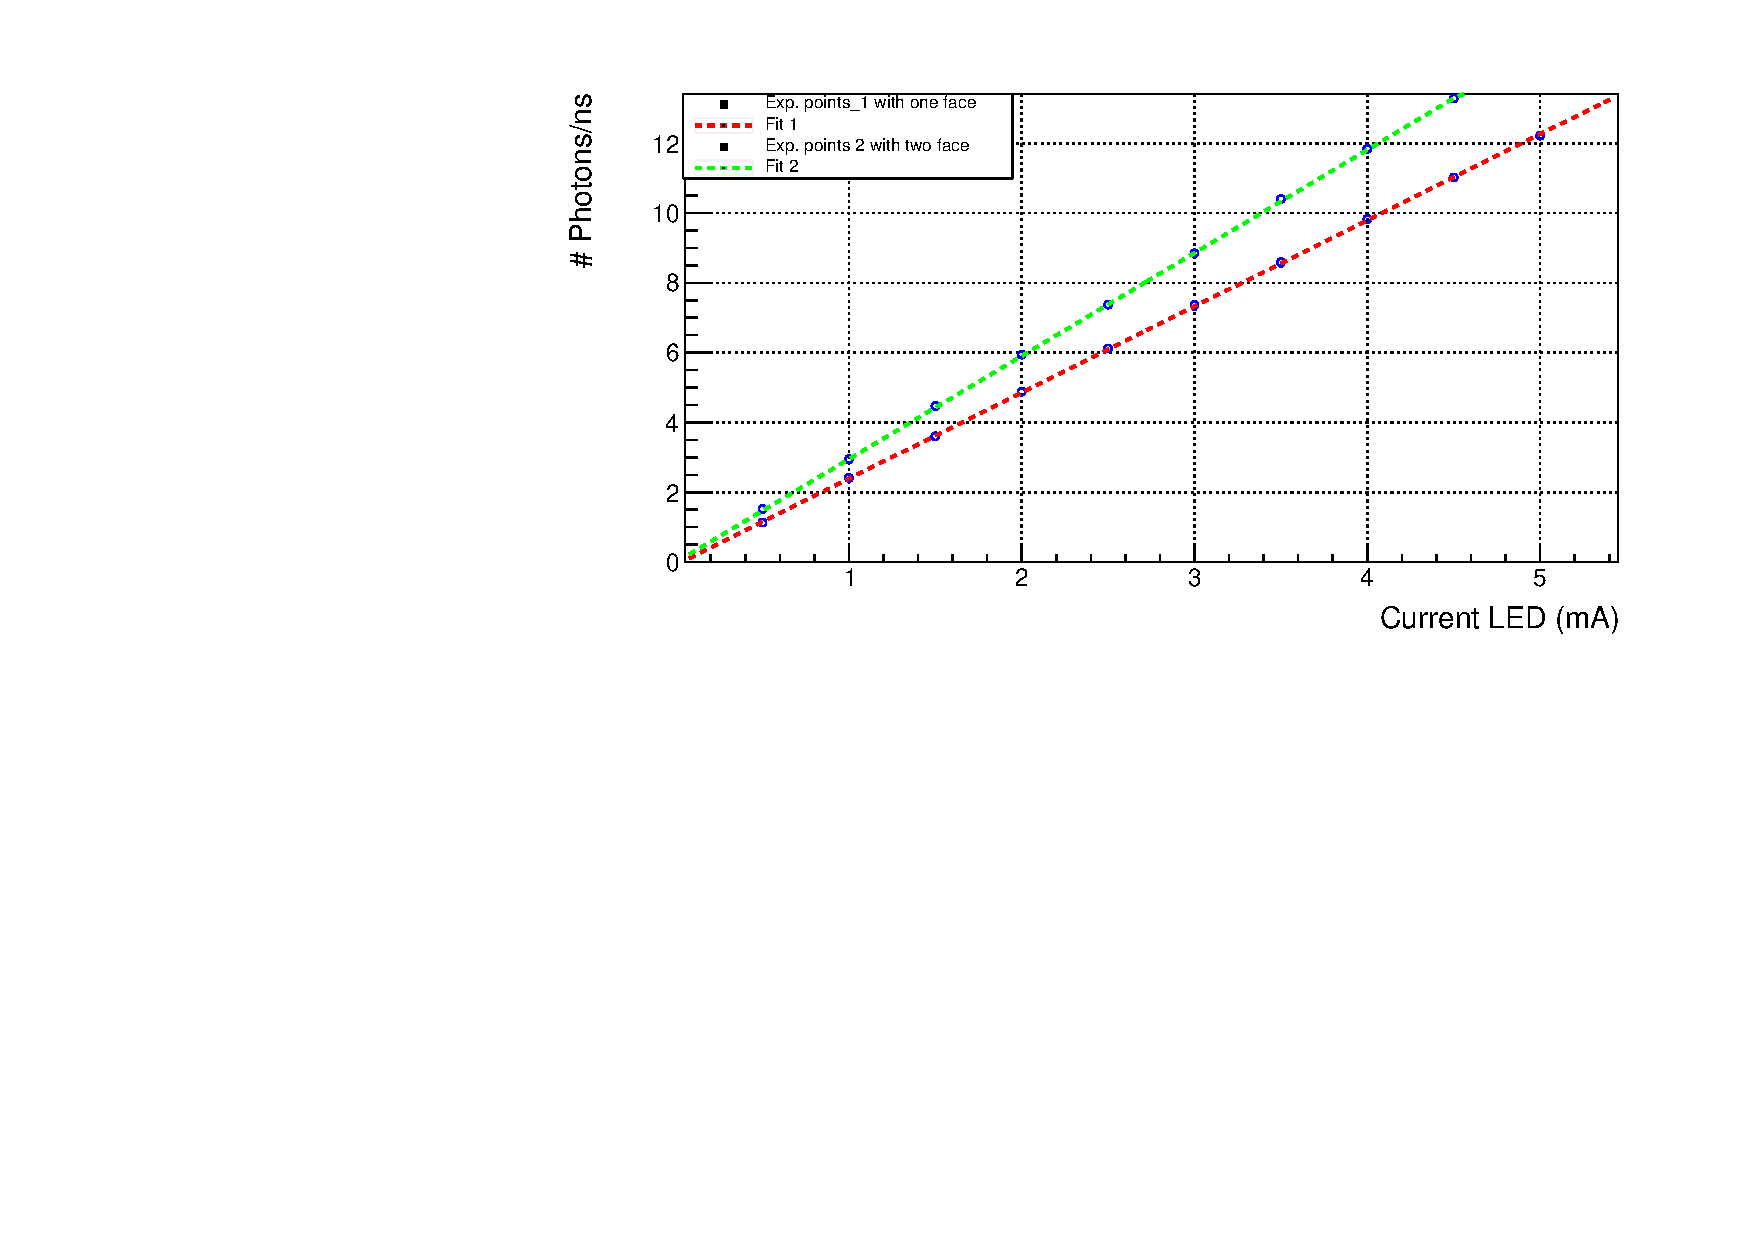
\includegraphics[scale=0.7]{Figuras/casefaces.pdf}
\caption{Intensidad promediada de 3 muestras diferentes de fibras no clad de $200~\mm$ frente a la alimentaicón de la LED con una cara pulida y con ambas.\label{resultadoscaras}}
\end{figure}

Seguidamente, en la figura \ref{diferenciacaras} se presenta la diferencia entre ambas señales:

\begin{figure}[hbtp]
\centering
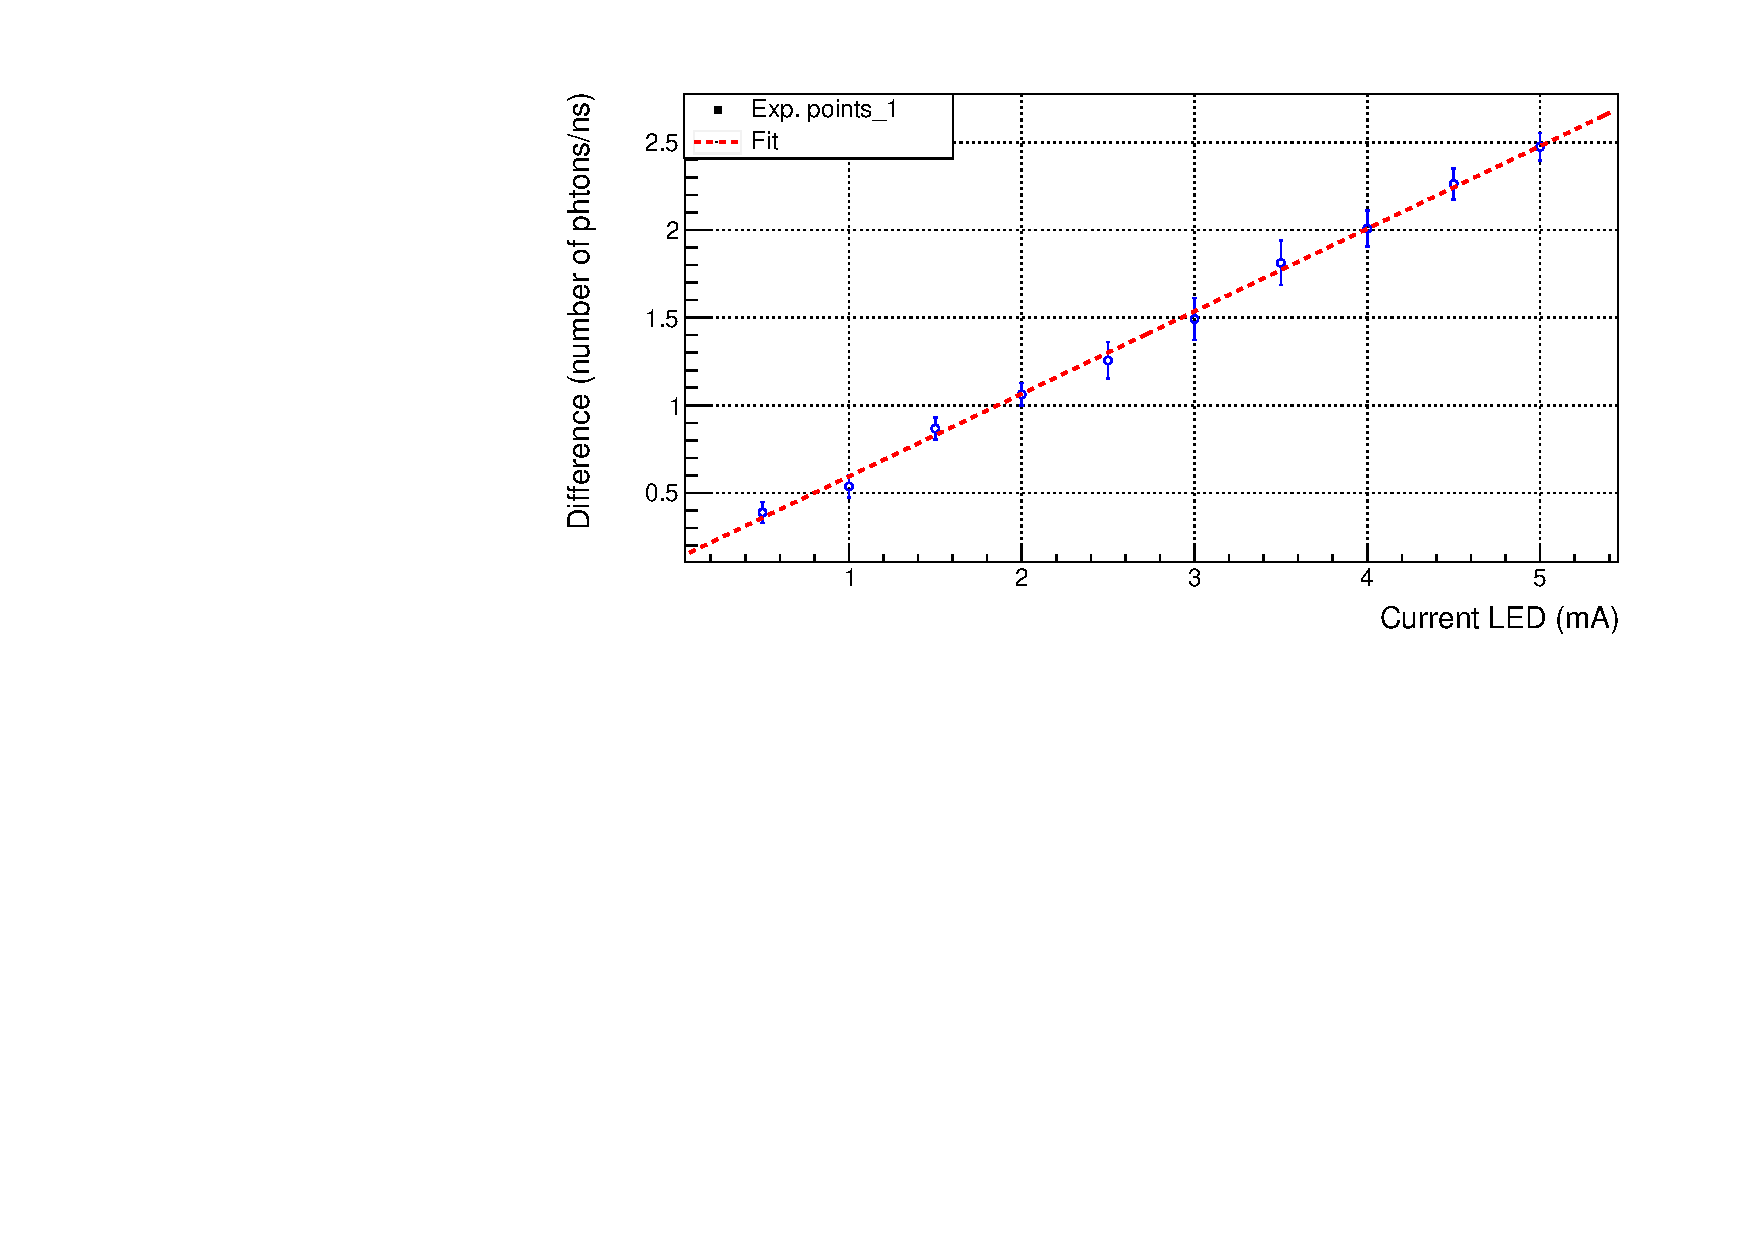
\includegraphics[scale=0.7]{Figuras/Differencefaces.pdf}
\caption{Diferencia entre las señales obtenidas de fibras no clad de $200~\mm$ frente a la alimentaicón de la LED con una cara pulida y con ambas.\label{diferenciacaras}}
\end{figure}

En esta figura podemos observar que, al nivel de señales de aproximadamente 12 fotones por nanosegundo (una tercera parte de las señales debida a eventos del tritio), ya observamos aproximadamente 2.5 fotones por nanosegundo menos en caso de no pulir ambas caras.

Por tanto, al nivel de las señales debidos a los eventos de tritio, si tenemos en cuenta la linealidad observada en el comportamiento, estimamos una perdida de aproximadamente 7.5 fotones por nanosegundo y por fibra. Si utilizamos centenares de fibras o incluso miles tendriamos pérdidas de 750 o 7500 respectivamente. Vemos por tanto que tendríamos una pérdida considerable de fotones, algo que no nos podemos permitir en el proyecto Tritium debido al hecho que ya estamos trabajando con señales excesivamente débiles. Debido a esto, las fibras utilizadas en el prototipo Tritium 1 se pulieron por ambas caras a pesar de realizarse la lectura únicamente por una.

Vemos por tanto que, a pesar de que el extremo se encuentra totalmente recubierto de teflon asegurando de esta manera una reflectividad de los fotones de casi el $100\%$, se necesita ademas un pulido de ambas caras evitando de esta forma una mayor dispersión de los fotones al llegar a este punto. 





\end{document}